\documentclass[12pt]{article}
\usepackage[utf8]{inputenc}
\usepackage{amsmath}
\usepackage[T1]{fontenc}

\title{ECE 3413 Lab 06\\*Stability of Loop Gain in a Negative Feedback System}
\author{Leomar Dur\'an}
\date{${29}^{\text{th}}$ March 2023}

\usepackage[natbib,style=apa6]{biblatex}
\addbibresource{main.bib}
\defbibheading{bibliography}[\refname]{%
  \section*{\centering #1}%
}%

\usepackage{hyperref}

\usepackage{cancel}
\usepackage[per-mode=symbol]{siunitx}
\newcommand*\siexpr[2][]{\SI[parse-numbers=false,#1]{#2}}%
\usepackage{xfrac}
\usepackage{amssymb}
\newcommand*\transpose{\mathsf{T}}

\usepackage{mathtools}%
\DeclarePairedDelimiter\brao()%
\DeclarePairedDelimiter\brac[]%
\DeclarePairedDelimiter\braco[)%
\DeclarePairedDelimiter\braoo][%
\DeclarePairedDelimiter\Brac\{\}%
\DeclarePairedDelimiter\abs||
\DeclarePairedDelimiter\norm\lVert\rVert%
\DeclarePairedDelimiter\piecefn\{.
\DeclarePairedDelimiter\evalat.|

\usepackage{lib/nonfloatenvirons}
\usepackage{booktabs}
\newcommand\ra[1]{\renewcommand*\arraystretch{#1}}
\ra{1.25}

\usepackage{minted}
\newcommand\matlab{matlab}

\usepackage{adjustbox}
\newcommand{\setprime}[2][1]{%
    {#2}^{%
        \raisebox{1pt}{%
            \scalebox{0.5}{%
                \itshape\sffamily\uppercase%
                \expandafter{%
                    \romannumeral#1%
                }%
            }%
        }
    }%
}%
\newcommand*\mcadj[7]%
% {#columns}{col spec}{rotation}{adjust spec}
% {before rotated text}{rotated text}{after rotated text}
{%
    \multicolumn{#1}{#2}{%
        \rlap{%
            #5\adjustbox{rotate=#3,#4}{#6}~#7%
        }%
    }%
}

\usepackage{pdfpages}
\usepackage{standalone}
\usepackage{matlab}

\usepackage[skip=\baselineskip,indent=0pt]{parskip}
\setlength\parindent{0pt}

\usepackage[shortlabels]{enumitem}

\def\hr{{\par\noindent\rule{\textwidth}{0.4pt}}}

\begin{document}

\maketitle
\newpage

\section{Introduction}

This is a two week lab.
Included are both week \texttt\#01 and week \texttt\#02.

The purpose of this lab in week 01 is to analyze a transfer function
and a set of modifications to that transfer function,
whether that be scaling the components of the poles, the natural frequency or adding poles.

This allows us to form relations between these parameters and the characteristics that we expect from a transfer function such as the transient response.

Not only can we estimate the effects that a modification will have on a transfer function, but we can use these relations to find new transfer functions just as one would pick components to have specific effects on a circuit.

In week 02, we also explore the damping of systems and feedback.

\section{Procedure}

\subsection{Task 1 -- Negative feedback system-equivalent transfer function}

Given the negative feedback system,

with
\begin{equation}
    \piecefn*{
        \begin{array}{@{}l@{}}
            \displaystyle
            G\brao*s = \frac{K}{s\brao{s + 2}^2},\\*
            H\brao*s = 1,
        \end{array}
    }
\end{equation}

the equivalent transfer function is
\begin{equation}
    \begin{aligned}
        \brao*{\frac{C}{R}}\brao*s
            &{}= \frac{G\brao*s}{1 + \brao*{GH}\brao*s}
    \\*
            &{}= \frac{1}{\displaystyle\sfrac1{G\brao*s} + H\brao*s}
    \\*
            &{}= \frac{1}{\displaystyle\brao*{\frac{s\brao*{s + 2}^2}K} + \brao*1} \times \frac{K}K
    \\*
            &{}= \frac{K}{s\brao*{s + 2}^2 + K}
    \\*
            &{}= \frac{K}{s^3 + 4s^2 + 4s + K}.
    \\*
    \end{aligned}
\end{equation}

\subsection{Task 2 -- Overdamped and underdamped systems}

\paragraph{To find an overdamped system,}%
first we must find the critical damping point.

This is found by first finding the characteristic equation, which is the denominator of the transfer function fix at $0$.
\begin{equation}
    s^3 + 4s^2 + 4s + K = 0.
\end{equation}

Let's generalize this characteristic equation with $p, q \in \mathbb{R}$ to
\begin{equation}
    s^3 + ps^2 + qs + K = 0.
\end{equation}

Then we solve for $K$.
\begin{equation}
    K = -s^3 - ps^2 - qs.
%    K = -s^3 - 4s^2 - 4s.
\end{equation}

We next find the fix the derivative of $K$ at $0$.
\begin{equation}
    0 = \evalat*{\frac{dK}{ds}}_{s=s_0} = -3s^2 - 2ps - q,
%   \evalat*{\frac{dK}{ds}}_{s=s_0} = -3s^2 - 8s - 4,
\end{equation}
and solve for $s_0$.
\begin{equation}
    s_{1,2} = %\brac*{\begin{matrix}
        \frac{+2p}{-6} \pm \frac{\sqrt{p^2 - 3q}}{-3}%
%        -2 \\* -\sfrac23
    %\end{matrix}}
    .
\end{equation}

After this point, the equation gets very complex and we will need to know the value of $K$ anyway. So let's substitute our coefficients $p = 4, q = 4$ into
\begin{equation}
    s_{1,2} = \brac*{\begin{matrix}
        -\sfrac63 \\* -\sfrac23
    \end{matrix}}%
    ,
\end{equation}
and solve for $K \not= 0$ again. This gives the critical damping point

\begin{equation}
    \Brac*{ K \middle| \brao*{K = \evalat*{\brao*{-s^3 - 4s^2 - 4s}}_{s \in s_{1,2}}}} \setminus \Brac0 = \Brac{\sfrac{32}{27}} \ni K_{\zeta=1}.
\end{equation}

Thus, if $K = \sfrac{32}{27} = K_{\zeta=1}$, then the system is critically damped. However, if $K < \sfrac{32}{27} = K_{\zeta=1}$, then the system is overdamped for overdamped systems.

Let's pick two gains $K = \sfrac{32}{27} - \SI4\percent = \sfrac{3072}{2700}$ and $K = \sfrac{32}{27} - \SI{10}\percent = \sfrac{2880}{2700}$.

\paragraph{To find an underdamped system}

We have a lower limit for a possibly underdamped system given above as $K_{\zeta=1}$.

To find the upper limit, we will need to use the Routh--Hurwitz criterion.

We start by making a table with one more rows as the degree of the denominator of the transfer function.
We populate the top two rows by alternatingly filling them with the coefficients of the denominator in order of descending degree.
If the last spot is empty, we fill it with $0$. We also add a last $0$ column.

\begin{table}[h]
    \centering
    \[
        \begin{array}{@{}*4r@{}}
            s^3: &                          1 & 4 & 0 \\*
            s^2: &                          4 & K & 0 \\*
%            s^1: &                          0 & 0 & 0 \\*
%            s^0: &                          0 & 0 & 0 \\*
        \end{array}
    \]
    \caption{First two rows of the Routh--Hurwitz table.}
    \label{tab:rh table 1st 2 rows}
\end{table}

Next we populate the remaining rows by filling each cell up to and including the penultimate of each column with the determinant of the $2\times2$ matrix formed by the first column and the column succeeding this column for the previous two rows, all divided by the first cell of the previous row.

For example, the first cell of row $s^1$ gets
$
    \dfrac14\abs*{
        \begin{matrix} 1 & 4 \\* 4 & K\end{matrix}
    } = 4 - K/4,
$

and the second cell of the same row gets
$
    \dfrac14\abs*{
        \begin{matrix} 1 & 0 \\* 4 & 0\end{matrix}
    } = 0.
$

The final column always gets $0$, resulting in the table.

\begin{table}[h]
    \centering
    \[
        \begin{array}{@{}*4r@{}}
            s^3: &                          1 & 4 & 0 \\*
            s^2: &                          4 & K & 0 \\*
            s^1: &                    4 - K/4 & 0 & 0 \\*
            s^0: & (K*(K - 16))/(4*(K/4 - 4)) & 0 & 0 \\*
        \end{array}
    \]
    \caption{The complete Routh--Hurwitz table.}
    \label{tab:rh table complete}
\end{table}

Next, we find the first row and corresponding $K$-values for which $\exists K$ s.t. the entire row is $0$.
The $K$-value of this first \textsc{zero} row is at the marginal stability point.

In row $s^1$, the value $K = 16$ gives $4 - K/4 = 4 - \brao*{16}/4 = 0$ thus giving the row $\begin{matrix}s^1: & 0 & 0 & 0\end{matrix}$.
Therefore the marginal stability point $K_{a=0} = 16$.

From the marginal stability point, we have that $K = 16 = K_{a=0}$ produces a system that is marginally stable and undamped, and we have that $K > 16 = K_{a=0}$ produces an unstable system.

Now if $K \in \braoo{\sfrac{32}{27}, \sfrac{432}{27}} = \braoo{K_{\zeta=1}, K_{a=0}}$, then the system is underdamped.

\subsection{Week 01, Part 01 -- Changing poles}\label{ssc:part 01}

\begin{enumerate}[(a)]
    \item
        Given the transfer function
        \begin{equation}
            G_2\brao*s = \frac{b}{s^2 + as + b},
        \end{equation}
        
        let the damping ratio and natural frequency, respectively $\zeta, \omega_n \in \mathbb{R}$ s.t. $a = 2\zeta\omega_n$ and $b = \omega_n^2$. So
        \begin{equation}
            \piecefn*{
                \begin{matrix}
                    \omega_n = \sqrt{b}\rlap, \\*
                    \zeta = \dfrac{a}{2\sqrt{b}}\rlap. \\*
                \end{matrix}
            }\rlap{$\qquad\brao*{b > 0}$}
        \end{equation}

        Furthermore
        \begin{equation}\label{eq:zwn}
            \zeta\omega_n = \frac{a}2,
        \end{equation}
        and
        \begin{equation}
            \sqrt{1 - \zeta^2} = \sqrt{1 - \brao*{\sfrac{a}{\brao*{2\sqrt{b}}}}^2} = \frac{1}{2\sqrt{b}} \sqrt{4b - a^2}.%
            \hskip1em\brao*{\abs*{a} \leq 2\sqrt{b}}
        \end{equation}
        
        We find that the peak time
        \begin{equation}\label{eq:peak time}
            T_p = \frac\pi{\omega_n \sqrt{1 - \zeta^2}} = \frac\pi{\brao*{\sqrt{b}}\brao*{ \frac{1}{2\sqrt{b}}\sqrt{4b - a^2}}} = \frac{2\pi}{\sqrt{4b - a^2}}.
        \end{equation}

        We find that the overshoot rate
        \begin{equation}\label{eq:overshoot}
            \begin{array}{*2{@{}r}@{}l@{}}\displaystyle
                \% OS
                &{}:={}& \exp\brao*{\frac{-\zeta\pi}{\sqrt{1 - \zeta^2}}} \SI{100}\percent
            \\*[1.3em]
                &{}={}& \exp\brao*{-\zeta\omega_n\brao*{\dfrac{\pi}{\omega_n\sqrt{1 - \zeta^2}}}} \SI{100}\percent
            \\*
                &{}={}& \exp\brao*{-\brao*{\zeta\omega_n}^{\vphantom{1}}T_p} \SI{100}\percent
            \\*
                &{}={}& \exp\brao*{-\brao*{\tfrac{a}2}^{\vphantom{1}}T_p} \SI{100}\percent
            \\*
                & {}={} & \exp\brao*{\dfrac{-aT_p}{2}} \SI{100}\percent\rlap.
            \\*
            \end{array}
        \end{equation}

        We find that the settling time
        \begin{equation}\label{eq:settling time}
            T_s \approx \frac4{\zeta\omega_n} = \frac4{\brao*{\sfrac{a}2}} = \frac8a.
        \end{equation}

        To find rise time, we must first find the step response in the time domain with parameters substituted.

        \subsubsection{Step response}
        We have
        \[
            G_2\brao*s = \frac{b}{s^2 + as + b},
        \]

        Well
        \begin{equation}
            C\brao*s = R\brao*s G_2\brao*s = \frac1s \frac{b}{s^2 + as + b}.
        \end{equation}

        So the second order factor of the denominator
        \begin{equation}\label{eq:sum of squares}
            \begin{aligned}
                s^2 + as + b
                &{} = \brao*{s^2 + 2\brao*{\frac{a}2}s + \brao*{\frac{a}2}^2} + \brao*{b - \brao*{\frac{a}2}^2}
            \\*
                &{} = \brao*{s + \frac{a}2}^2 + \brao*{\sqrt{b - \brao*{\frac{a}2}^2}}^2
                \rlap{
                    $\hskip0.5em\brao*{\abs*{a} \leq 2\sqrt{b}}$
                }
            \\*
                &{}= \brao*{s + \hat{a}}^2 + \omega_d^2.
            \\*
            \end{aligned}
        \end{equation}

        Thus, for $G_2\brao*s$, we have exponential and the damped frequencies
        \begin{equation}\label{eq:Laplace constants}
            \piecefn*{
                \begin{array}{@{}l@{}}
                    \displaystyle
                    \hat{a} = \frac{a}2, \\*
                    \omega_d = \sqrt{b - \hat{a}^2}. \\*
                \end{array}
            }
        \end{equation}

        \paragraph{Note that} the damped frequency and peak time respectively
        \begin{equation}\label{eq: w to-from Tp}
            \begin{array}{c}
            \displaystyle
                \omega_d = \frac\pi{\sfrac{2\pi}{\sqrt{4b - a^2}}} = \frac\pi{T_p}.
            \\*
            \midrule\midrule
            \displaystyle
                T_p = \frac\pi\omega_d.
            \\*
            \end{array}
        \end{equation}

        Thus, we find coefficients $A,B,C$ s.t.
        \begin{equation}
            b = A\brao{s^2 + as + b} + B\brao{s^2 + \hat{a}s} + C\omega_d s.
        \end{equation}

        Assume $s = 0$. Then
        \begin{equation}
            s = 0: b = A\brao{\cancel{\brao*0^2} + \cancel{a\brao*0} + b} + B\brao*{\cancel{\brao*0^2} + \cancel{\hat{a}\brao*0}} + \cancel{C\omega_d \brao*0}.
        \end{equation}
        So $b = Ab$. Thus $A = 1$. Thus
        \begin{equation}
            b = \brao{s^2 + as + b} + B\brao{s^2 + \hat{a}s} + C\omega_d s.
        \end{equation}
        For quadratic terms, we have $0s^2 = s^2 + Bs^2$. So $B = -1$. Thus
        \begin{equation}
            b = \brao{s^2 + as + b} - \brao{s^2 + \hat{a}s} + C\omega_d s.
        \end{equation}
        Finally, for linear terms, we have $0s = as - \hat{a}s + C\omega_d s$. Thus
        \begin{equation}
            C = \frac{\hat{a} - a}\omega_d
            = \frac{\displaystyle\brao*{\frac{a}2} - a}\omega_d
            = \frac{-a}{2\omega_d},\ 
            % = \frac{\displaystyle\brao*{\frac{a}2} - a}{\displaystyle\sqrt{b - \brao*{\frac{a}2}^2} } = \frac{-a}{\sqrt{4b - a^2}}.
            \omega_d = \sqrt{b - \brao*{\frac{a}2}^2} \not= 0.
        \end{equation}

        Then by the inverse Laplace transform, in the time domain, we have step response
        \begin{equation}
            \begin{aligned}
                c\brao*t = \brao*{1 + \brao*{-\cos\brao{\omega_d t} - \frac{a}{2\omega_d} \sin\brao{\omega_d t} }{e^{-\brao*{\sfrac{a}2}t}}}u\brao*t,
            \end{aligned}
        \end{equation}
        given $\displaystyle
            \omega_d = \sqrt{b - \brao*{\frac{a}2}^2}.
        $

        After this step, we cannot solve the general case for $t$. So we must first evaluate $c\brao*t$ at some values for $a, \omega_d$.

        \subsubsection{Evaluations}\label{sss:evaluations}
        Let's evaluate at $a = 4, b = 25$. Well
        \begin{equation}
            \piecefn*{
                \begin{array}{@{}l@{}}
                    b = \brao*{25} > 0,
                \\*
                    \abs{a} = \abs{4} = 4 < 10 = 2\sqrt{\brao{25}} = 2\sqrt{b},
                \\*
                    \omega_d = \sqrt{\brao{25} - \brao*{\dfrac{\brao*4}2}^2} = \sqrt{21} \not= 0
                \\*
                \end{array}
            }
        \end{equation}
        The peak time
        \begin{equation}
            T_p = \frac\pi{\sqrt{21}} = \siexpr{0.6\overline956}\second.
        \end{equation}
        The overshoot rate
        \begin{equation}
                \% OS
                ={} \exp\brao*{\frac{-\brao4\brao{\SI{0.6856}\second}}2} \SI{100}\percent
                = \brao*{0.2\overline53\,802}{\SI{100}\percent}
                = \siexpr{2\overline5.3802}\percent.
        \end{equation}
        The setting time
        \begin{equation}
            T_s \approx \frac84 = \SI2\second.
        \end{equation}

        For the rise time, in the time domain, the step response
        \begin{equation}
            \begin{aligned}
                c\brao*t = \brao*{1 + \brao*{-\cos\brao{\omega_d t} - \frac{a}{2\omega_d} \sin\brao{\omega_d t} }{e^{-\brao*{\sfrac{a}2}t}}}u\brao*t.
            \end{aligned}
        \end{equation}

        Assuming that $a > 0$, then the final value is s.t.
        \begin{equation}
            c\brao*t
            \xrightarrow{t\to+\infty} \brao*{1 + \brao*{-\cos\brao{\omega_d t} - \frac{a}{2\omega_d} \sin\brao{\omega_d t} }\cancel{\brao*{e^{-\brao*{\sfrac{a}2}t}}}^0} \cancel{u\brao*t}^1 =\!1\!=\!c_f.
        \end{equation}

        Thus, the $\SI{90}\percent$ and $\SI{10}\percent$ values are $.9c_f = 0.9$ and $.1c_f = 0.1$ respectively.

        Well $a = 4,\ \omega_d = \sqrt{21} \not= 0$.
        Using these known values, we can use the script in Appendix subsection~\ref{sap:solving for .9cf and .1cf}, we find the times corresponding to these values
        \begin{equation}
            \brac*{
                \begin{matrix}
                    t_{.9f} \\*
                    t_{.1f} \\*
                \end{matrix}
            }
            =
            \brac*{
                \begin{matrix}
                    \SI{0.388761}\second \\*
                    \SI{0.096063}\second \\*
                \end{matrix}
            }\rlap.
        \end{equation}
        Thus, rise time $T_r = t_{.9f} - t_{.1f} = \SI{0.388761}\second - \SI{0.096063}\second = \SI{0.292698}\second$.

        \subsubsection{Plotting the poles and zeroes}\label{sss:poles-zeros}

        In \eqref{eq:sum of squares}, we found that the denominator of transfer function $G_2\brao*s$ is $s^2 + as + b = \brao{s + \hat{a}}^2 + \omega_d^2$.

        Thus the poles $s$ s.t.
        \begin{equation}
            \begin{aligned}
                0 &{}= \brao*{s + \hat{a}}^2 + \omega_d^2
            \\*
                  &{}= \brao*{s + \hat{a}}^2 - \brao*{j\omega_d}^2
            \\*
                  &{}= \brao*{s + \brao*{\hat{a} - j\omega_d}}\brao*{s + \brao*{\hat{a} + j\omega_d}},
            \\*
            \end{aligned}
        \end{equation}
        that is
        \begin{equation}\label{eq:poles}
            \begin{aligned}
                s_{1,2} = -\hat{a} \pm j\omega_d
            %\\*
                = -\frac{a}2 \pm j\omega_d
                \rlap.
            %\\*
            \end{aligned}
        \end{equation}

        Substituting in the parameters, the poles
        \begin{equation}
            s_{1,2} = -\frac42 \pm j\sqrt{21} = -2 \pm j\sqrt{21}\rlap.
        \end{equation}

        Now, although the poles and zeros may be plotted with the built-in Matlab function \mintinline\matlab{pzmap}, which accepts a transfer function or system and plots its zeroes and poles,
        I have written the Matlab script in Appendix subsection~\ref{sap:pzplot} showing how it works with results in Fig.~\ref{fig:part01_pzplot_pzmap}.

    \item
        \subsubsection{Effect of the pole's real and imaginary parts}
        \paragraph{On the parameters}
        From \eqref{eq:poles} and since $\abs*{a} \leq 2\sqrt{b}$, $\omega_d\in\mathbb{R}$. So let $s_0\in s_{1,2}$, then $s_{1,2} = \mathfrak{Re}\brao*{s_0} \pm j\mathfrak{Im}\brao*{s_0}$ and
        the real part of $s_0$,
        \begin{equation}\label{eq:Re(s0)}
            \mathfrak{Re}\brao*{s_0} := \frac{s_1 + s_2}2
            %= -\hat{a}
            = -\frac{a}2\rlap,
        \end{equation}
        and the imaginary part
        \begin{equation}\label{eq:Im(s0)}
            \mathfrak{Im}\brao*{s_0} := \abs*{\frac{s_1 - s_2}{2j}} = \omega_d = \sqrt{b - \hat{a}^2} = \sqrt{b - \brao*{\frac{a}2}^2}\rlap.
        \end{equation}

        Thus, we have parameters $a,b$ s.t. $a = -2 \mathfrak{Re}\brao*{s_0}$, and
        \begin{equation}
            \begin{aligned}
                b &{}= \mathfrak{Im}^2\brao*{s_0} + \hat{a}^2
            \\*
                & {}= \mathfrak{Im}^2\brao*{s_0} + \brao*{-\mathfrak{Re}\brao*{s_0}}^2
            \\*
                & {}= \brao*{\mathfrak{Re}^2 + \mathfrak{Im}^2}\brao*{s_0}.
            \\*
            \end{aligned}
        \end{equation}

        Let $m,n \in \mathbb{R}$, and let $\setprime{s}_0 \in \setprime{s}_{1,2} = m\mathfrak{Re}\brao*{s_0} \pm jn\mathfrak{Im}\brao*{s_0}$ s.t.
        \begin{equation}
            \piecefn*{
                \begin{matrix}
                    \mathfrak{Re}\brao*{\setprime{s}_0} = m\mathfrak{Re}\brao*{s_0},
                \\*
                    \mathfrak{Im}\brao*{\setprime{s}_0} = n\mathfrak{Im}\brao*{s_0}.
                \\*
                \end{matrix}
            }
        \end{equation}

        Thus the new parameters,
        \begin{equation}
            \piecefn*{
                \begin{array}{@{}l@{}}\displaystyle
                      \setprime{a}
                    = -2\mathfrak{Re}\brao*{\setprime{s}_0}
                    = -2m\mathfrak{Re}\brao*{s_0}
                    \rlap,
                \\*
                      \setprime{b}
                    = \brao*{\mathfrak{Re}^2 + \mathfrak{Im}^2}\brao*{\setprime{s}_0}
                    = \brao*{\brao*{\tilde{m}\mathfrak{Re}}^2 + \tilde{n}^2\mathfrak{Im}^2}\brao*{s_0}
                    \rlap.
                \\*
                \end{array}
            }
        \end{equation}

        Further, in comparison with the original parameters,
        the new parameters
        \begin{equation}
            \piecefn*{
                \begin{array}{@{}l@{}}\displaystyle
                      \setprime{a}
                    = -2m\brao*{-\frac{a}2}
                    = ma
                    \rlap,
                \\*\displaystyle
                      \setprime{b}
                    = \brao*{\brao*{\brao*m\brao*{-\frac{a}2}}^2 + n^2\brao*{\sqrt{b - \brao*{\frac{a}2}^2}}^2}
                    = \brao*{m^2 - n^2}\brao*{\frac{a}2}^2 + n^2 b
                    \rlap.
                \\*
                \end{array}
            }
        \end{equation}

        \paragraph{On step response characteristics}
        From \eqref{eq: w to-from Tp}, we have peak time
        \begin{equation}\label{eq:peak time, m, n}
            \begin{aligned}
                      \setprime{T}_p
                &{} = \frac\pi{\mathfrak{Im}\brao*{\setprime{s}_0}}
            \\*
                &{} = \frac\pi{n\mathfrak{Im}\brao*{s_0}}
            \\*
                &{} = \frac1n\brao*{\frac\pi{\mathfrak{Im}\brao*{s_0}}}
            \\*
                &{} = \frac{T_p}n
            \\*
                % &{}= \frac{2\pi}{\sqrt{4\setprime{b} - \brao*{\setprime{a}}^2}}
            % \\*
                % &{}= \frac{2\pi}{\sqrt{4\brao*{\brao*{m^2 - n^2}\brao*{\dfrac{a}2}^2 + n^2 b} - \brao*{ma}^2}}
            % \\*
                % &{}= \frac{2\pi}{\abs*n\sqrt{4b - a^2}}
            % \\*
                % &{}= \frac1{\abs*n} \brao*{\frac{2\pi}{\sqrt{4b - a^2}}}
            % \\*
                % &{}= \frac{T_p}{\abs*n}.
            % \\*
            \end{aligned}
        \end{equation}

        From \eqref{eq:overshoot}, we have the rate of overshoot
        \begin{equation}\label{eq:overshoot, m, n}
            \begin{aligned}
                \%\setprime{OS} &{}= \exp\brao*{\dfrac{-\brao*{\setprime{a}}T_p}{2}} \SI{100}\percent
            \\*
                     &{}= \exp\brao*{\dfrac{-\brao*{ma}T_p}{2}} \SI{100}\percent
            \\*
                     &{}= \exp\brao*{\dfrac{-ma T_p}{2}} \SI{100}\percent.
            \\*
                     &{}= \brao*{\frac{\exp\brao*{\dfrac{-a T_p}{2}}\SI{100}\percent}{\SI{100}\percent}}^m \SI{100}\percent.
            \\*
                     &{}= \brao*{\frac{\%OS}{\SI{100}\percent}}^m \SI{100}\percent.
            \\*
            \end{aligned}
        \end{equation}

        From \eqref{eq:settling time}, we have the settling time
        \begin{equation}\label{eq:settling time, m, n}
            \setprime{T}_s \approx \frac8{\setprime{a}} = \frac8{ma} = \frac1m\brao*{\frac8{a}} = \frac{T_s}m.
        \end{equation}

        As stated before, the relationship between parameters $a, b$ and therefore the poles of the transfer function and the rise time are too complicated to calculate in a general form.

        \paragraph{Evaluations on the real part}

        Suppose that we modified the poles, so that the imaginary part stays the same, and the real part is $2\times$.
        So $m = 2,\ n = 1$
        and the roots $\setprime{s}_{1,2} = 2\brao*{-2} \pm j\sqrt{21} = -4 \pm j\sqrt{21}$%
        , plotted in Fig.~\ref{fig:part01_pzplot_pzmap}%
        .
        Then we have the parameters
        \begin{equation}
            \piecefn*{
                \begin{array}{@{}l@{}}\displaystyle
                    \setprime{a} = ma = \brao2\brao4 = 8,
                \\*\displaystyle
                      \setprime{b}
                    = \brao*{m^2 - n^2}\brao*{\frac{a}2}^2 + n^2b
                    = \brao*{\brao2^2 - \brao1^2}\brao*{\frac{\brao4}2}^2 + \brao1^2\brao{25}
                    = 37\rlap.
                \end{array}
            }
        \end{equation}

        Thus the new transfer function
        \begin{equation}
            \setprime{G}_2\brao*s := \frac{37}{s^2 + 8s + 37},
        \end{equation}
        which is used to plot the pole-zero map in Fig.~\ref{fig:part01_pzplot_pzmap}, generated by the Matlab statement \mintinline\matlab{pzmap(tf(29, [1 8 29]))}

        We saw that peak time is independent of $m$.
        Thus $\setprime{T}_p = T_p = \siexpr{0.6\overline956}\second$. Now
        the rate of overshoot
        \begin{equation}
            \begin{aligned}
                  \%\setprime{OS}
                &{}= \brao*{\frac{\brao*{\brao*{0.2\overline53\,802}\cancel{{\SI{100}\percent}}^{\,1}}}{\cancel{\SI{100}\percent}^{\,1}}}^{\brao*{2}} \SI{100}\percent
            \\*
                &{}= \brao*{0.06\overline4\,415} \SI{100}\percent
            \\*
                &{}= \siexpr{6.\overline4415}\percent.
            \\*
            \end{aligned}
        \end{equation}
        and the settling time
        \begin{equation}
            \setprime{T}_s
            \approx \frac{\brao*{\SI2\second}}{\brao2}
            = \SI1\second.
        \end{equation}

        Now for rise time, we have $\setprime{a} = 8$ and $\setprime\omega_d = \mathfrak{Im}\brao*{\setprime{s}_0} = \sqrt{21}$.
        Thus, the Matlab script in Appendix subsection~\ref{sap:solving for .9cf and .1cf} produces the limits
        \begin{equation}
            \brac*{
                \begin{matrix}
                    \setprime{t}_{.9f} \\*
                    \setprime{t}_{.1f} \\*
                \end{matrix}
            }
            =
            \brac*{
                \begin{matrix}
                    \SI{0.411704}\second \\*
                    \SI{0.082401}\second \\*
                \end{matrix}
            }\rlap,
        \end{equation}
        and rise time $\setprime{T}_r = \SI{0.411704}\second - \SI{0.082401}\second = \SI{0.329303}\second$.

    \item
        \subsubsection{Effect of the pole's imaginary part}
        This time, let's modified the poles, so that the real part stays the same, and the imaginary part is $\frac12\times$.
        So $m = 1,\ n = \sfrac12$
        and the roots $\setprime[2]s_{1,2} = -2 \pm j\brao{\sfrac12}\sqrt{21}$
        , plotted in Fig.~\ref{fig:part01_pzplot_pzmap}%
        . The parameters
        \begin{equation}
            \piecefn*{
                \begin{array}{@{}l@{}}\displaystyle
                    \setprime[2]a = ma = \brao1\brao4 = 4,
                \\*\displaystyle
                      \setprime[2]b
                    = \brao*{m^2 - n^2}\brao*{\frac{a}2}^2 + n^2b
                    = \brao*{\brao1^2 - \brao*{\sfrac12}^2}\brao*{\frac{\brao4}2}^2 + \brao*{\sfrac12}^2\brao{25}
                    = \sfrac{37}4\rlap.
                \end{array}
            }
        \end{equation}

        So the transfer function is
        \begin{equation}
            \setprime[2]{G}_2\brao*s = \frac{\sfrac{37}4}{s^2 + 4s + \tfrac{37}4}.
        \end{equation}

        From \eqref{eq:peak time, m, n}, the peak time
        \begin{equation}
            \setprime[2]{T}_p = \frac{\siexpr{0.6\overline956}\second}{\brao*{\sfrac12}} = \siexpr{1.\overline4712}\second.
        \end{equation}
        In \eqref{eq:overshoot, m, n}, \eqref{eq:settling time, m, n},
        we see that $\%OS,\ T_s$ are independent of $n$.
        Thus $\%\setprime[2]{OS} = \%OS = \siexpr{2\overline5.3802}\percent$ and $\setprime[2]{T}_s \approx T_s \approx \SI2\second$.

        Again for rise time, we have $\setprime[2]a = 4$ and $\setprime[2]\omega_d = \mathfrak{Im}\brao*{\setprime[2]s_0} = \brao*{\sfrac12}\sqrt{21}$.
        Thus, the Matlab script in Appendix subsection~\ref{sap:solving for .9cf and .1cf} produces the limits
        \begin{equation}
            \brac*{
                \begin{matrix}
                    \setprime[2]t_{.9f} \\*
                    \setprime[2]t_{.1f} \\*
                \end{matrix}
            }
            =
            \brac*{
                \begin{matrix}
                    \SI{0.823409}\second \\*
                    \SI{0.164802}\second \\*
                \end{matrix}
            }\rlap,
        \end{equation}
        and rise time $\setprime[2]T_r = \SI{0.823409}\second - \SI{0.164802}\second = \SI{0.658607}\second$.

    \item
        \subsubsection{Effect of the natural frequency}

        \paragraph{On the parameters}
        As we defined earlier, $a = 2\zeta\omega_n$ and $b = \omega_n^2$.
        Let $\nu \in \mathbb{R}$ and let $\setprime[3]\omega_n = \nu\omega_n$.
        Thus
        \begin{equation}
            \piecefn*{
                \begin{array}{@{}l@{}}
                    \setprime[3]a = 2\zeta\setprime[3]\omega_n = 2\zeta\nu\omega_n = \nu\brao{2\zeta\omega_n} = \nu a,
                \\*
                    \setprime[3]b = \brao*{\setprime[3]\omega_n}^2 = \brao*{\nu\omega_n}^2 = \nu^2 b.
                \\*
                \end{array}
            }
        \end{equation}

        \paragraph{On step response characteristics}
        From \eqref{eq:peak time}, \eqref{eq: w to-from Tp},
        the damped frequency for the inverse Laplace transform,
        \begin{equation}
              \omega_d = \omega_n\sqrt{1 - \zeta^2}.
        \end{equation}
        So the new damped frequency
        \begin{equation}
              \setprime[3]\omega_d
            = \setprime[3]\omega_n\sqrt{1 - \zeta^2}
            = \brao*{\nu\omega_n}\sqrt{1 - \zeta^2}
            = \nu\omega_d\rlap.
        \end{equation}
        From \eqref{eq:peak time}, we have peak time
        \begin{equation}
              \setprime[3]T_p
            = \frac\pi{\setprime[3]\omega_d}
            = \frac\pi{\nu\omega_d}
            = \frac1\nu\brao*{\frac\pi\omega_d}
            = \frac{T_p}\nu\rlap.
            % = \frac\pi{\setprime[3]\omega_n \sqrt{1 - \zeta^2}}
            % = \frac\pi{\nu\omega_n \sqrt{1 - \zeta^2}}
            % = \frac1\nu \brao*{\frac\pi{\omega_n \sqrt{1 - \zeta^2}}}
            % = \frac{T_p}\nu\rlap.
        \end{equation}
        From \eqref{eq:overshoot}, we have rate of overshoot
        \begin{equation}
              \%\setprime[3]{OS}
            = \exp\brao*{\frac{-\zeta\pi}{\sqrt{1 - \zeta^2}}} \SI{100}\percent
            = \%OS.
        \end{equation}
        Thus, we see that the natural frequency has no effect on the overshoot.
        However, from \eqref{eq:settling time}, we have settling time
        \begin{equation}
                    \setprime[3]T_s
            \approx \frac4{\zeta\setprime[3]\omega_n}
                  = \frac4{\zeta\brao*{\nu\omega_n}}
                  = \frac1\nu \brao*{\frac4{\zeta\nu\omega_n}}
                  = \frac{T_s}\nu.
        \end{equation}

        \paragraph{Evaluations}
        Suppose that we modify the natural frequency so that it is $4\times$.
        So $\nu = 4$. Thus we have parameters
        \begin{equation}
            \piecefn*{
                \begin{array}{@{}l@{}}
                    \setprime[3]a = \brao*4\brao*4 = 16,
                \\*
                    \setprime[3]b = \brao*4^2 \brao*{25} = 400.
                \\*
                \end{array}
            }
        \end{equation}
        Thus the transfer function
        \begin{equation}
            \setprime[3]G_2\brao*s = \frac{400}{s^2 + 16 + 400}.
        \end{equation}

        So the peak time
        \begin{equation}
              \setprime[3]T_p
            = \frac{\brao{\siexpr{0.6\overline956}\second}}{4}
            = \siexpr{0.1\overline714}\second\rlap,
        \end{equation}
        the rate of overshoot, which is independent of the natural frequency,
        $\%\setprime[3]{OS} = \%OS = \siexpr{2\overline5.3802}\percent$
        and the settling time
        \begin{equation}
                    \setprime[3]T_s
            \approx \frac{\SI2\second}4
                  = \SI{0.5}\second.
        \end{equation}

        From $\setprime[3]a = 16$, $\setprime[3]\omega_d = \brao*{4}\brao*{\sqrt{21}} = 4\sqrt{21}$,
        using the script in Appendix subsection~\ref{sap:solving for .9cf and .1cf},
        we find the limits of the rise time
        \begin{equation}
            \brac*{
                \begin{matrix}
                    \setprime[3]t_{.9f} \\*
                    \setprime[3]t_{.1f} \\*
                \end{matrix}
            }
            =
            \brac*{
                \begin{matrix}
                    \SI{0.097190}\second \\*
                    \SI{0.024016}\second \\*
                \end{matrix}
            }\rlap.
        \end{equation}
        Thus the rise time $\setprime[3]T_r = \SI{0.097190}\second - \SI{0.024016}\second = \SI{0.073175}\second$.

        As for the poles, from \eqref{eq:zwn}, \eqref{eq:Re(s0)},
        \begin{equation}
            \mathfrak{Re}\brao*{s_0} = -\zeta\omega_n,
        \end{equation}
        and with \eqref{eq:Im(s0)}, the poles
        \begin{equation}
            s_{1,2} = -\zeta\omega_n \pm j\omega_d.
        \end{equation}
        So the new poles
        \begin{equation}
              \setprime[3]s_{1,2}
            = -\zeta\setprime[3]\omega_n \pm j\setprime[3]\omega_d
            = -\zeta\brao*{\nu\omega_n} \pm j\brao*{\nu\omega_d}
            = \nu\brao*{-\zeta\omega_n \pm j\omega_d}
            = \nu s_{1,2}.
        \end{equation}
        Thus $\mathfrak{Re}\brao*{\setprime[3]s_0} = \nu\mathfrak{Re}\brao*{s_0}$
        and $\mathfrak{Im}\brao*{\setprime[3]s_0} = \nu\mathfrak{Im}\brao*{s_0}$.
\end{enumerate}

\subsection{Week 01, Part 02 -- Adding poles}

As \citet{nise2015a} warns,
the step response formulas in \ref{eq:peak time}, \ref{eq:overshoot}, \ref{eq:settling time} are designed only for second order transfer functions with no zeros.
When a transfer function falls outside of those parameters, there are other techniques to analyze it.

\begin{enumerate}[(a)]
    \item
        \subsubsection{Non-positive real pole with great magnitude}

        If the extra pole is a real, non-positive $-\alpha_{{R}} \in \mathbb{R}_{\leq 0}$ and has a magnitude much greater than that of the real part of the second order poles,
        then the step response of the transfer function can be approximated by ignoring this extra real pole.

        This is the case with adding the pole $-\alpha_R = -200$, since $+\alpha_R = 200 \gg 2 = \abs*{\mathfrak{Re}\brao*{s_0}}$ of the pole that we found in sub-subsection~\ref{sss:poles-zeros}.

    \item
        \subsubsection{Positive real pole}

        Now, if the pole is a real and positive pole $+\alpha_R \in \mathbb{R}_{> 0}$, then this pole adds an addend $\frac{D}{s - \alpha_R}$ to the partial fraction decomposition as in
        \begin{equation}
            C\brao*s = \frac{A}s + \frac{B\brao*{s + \hat{a}}+ C\omega_d}{\brao*{s + \hat{a}}^2 + \omega_d^2} + \frac{D}{s - \alpha_R}.
        \end{equation}

        In the time domain, this addend produces a growing exponential
        \begin{equation}
            c\brao*t = \brao*{
                A + \brao*{
                      B\cos\brao*{\omega_d t}
                    + C\sin\brao*{\omega_d t}^{\vphantom{1}}
                }^{\vphantom{1}}
                e^{-\hat{a}t}
                + De^{\alpha_Rt}
            }u\brao*t
        \end{equation}

        Now we know that
        \begin{equation}
            \brao*{
                A + \brao*{
                      B\cos\brao*{\omega_d t}
                    + C\sin\brao*{\omega_d t}^{\vphantom{1}}
                }^{\vphantom{1}}
                \cancel{\brao*{e^{-\hat{a}t}}}^0
            }\cancel{u\brao*t}^1
            \xrightarrow{t\to+\infty} A.
        \end{equation}
        However
        \begin{equation}
            \brao*{
                De^{\alpha_Rt}
            }
            \xrightarrow{t\to+\infty} +\infty,
        \end{equation}
        that is, the growing exponential component goes to infinity. Thus so does $c\brao*t$ since $\lim_{h\to+\infty} A + h = \lim_{h\to+\infty} h$.
        Because of that, the new transfer function is unstable.
\end{enumerate}

\subsection{Week 02, Part 01(a) -- Poles and damping of systems}

Suppose we have the transfer functions

\begin{equation}
    G_1 := \frac{400}{s^2 + 12s + 400}.
\end{equation}

\begin{figure}
    \centering
    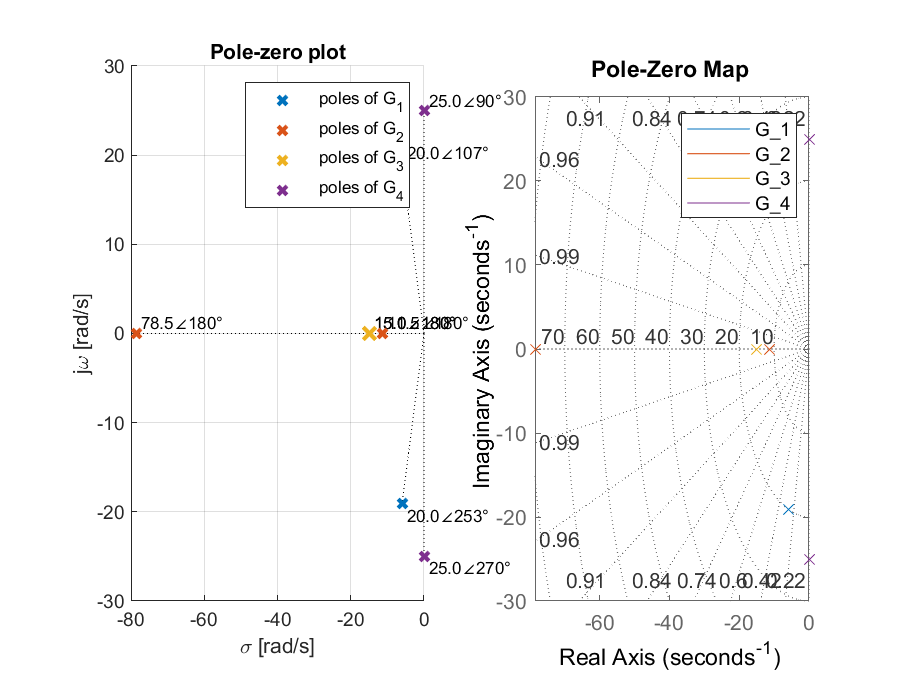
\includegraphics[width=\linewidth]{img/w02_part01a_pzplot.eps}
    \caption{Pole-zero plot of the transfer functions $G_1, G_2, G_3, G_4$ using both my custom plot on the left and Matlab's built-in \mintinline\matlab{pzmap} function on the right}
    \label{fig:w02 pzplot}
\end{figure}

\begin{equation}
    G_2 := \frac{900}{s^2 + 90s + 900}.
\end{equation}

\begin{equation}
    G_3 := \frac{225}{s^2 + 30s + 225}.
\end{equation}

\begin{equation}
    G_4 := \frac{625}{s^2 + 625}.
\end{equation}

As we did in sub-subsection~\ref{sss:poles-zeros},
let us use a Matlab script similar to the one in Appendix subsection~\ref{sap:pzplot}
with the only difference being the transfer functions and their labels.
The modified script is included in Appendix subsection~\ref{sap:pzplot 2}.
It produces the pole-zero plot in Fig.~\ref{fig:w02 pzplot}.

From the pole-zero plots, let's make some predictions about the systems.
\begin{enumerate}
    \item
        The poles of $G_1$, $s_{\brao*{11},\brao*{12}} = -6 \pm j\sqrt{364}$
        are on the left half plane, but not on the $x$-axis.
        They
        have negative real part and nonzero imaginary part.
        Thus the system of $G_1$ is stable and underdamped.
    \item
        The poles of $G_2$, $s_{\brao*{21},\brao*{22}} = -45 \pm \sqrt{1125}$
        are on the left half $x$-axis and not coincident.
        They
        have negative real part and zero imaginary part, but are a unique pair of roots.
        Thus the system of $G_2$ is stable and overdamped.
    \item
        The poles of $G_3$, $s_{\brao*{21},\brao*{22}} = -15 \pm 0$
        are on the left half $x$-axis and coincident.
        They
        have negative real part, zero imaginary part and are in fact a double root.
        Thus the system of $G_3$ is stable and critically damped.
    \item
        The poles of $G_4$, $s_{\brao*{21},\brao*{22}} = \pm j\sqrt{625}$
        are on the $y$-axis, but not on the origin.
        They
        have zero real part and are in fact purely imaginary.
        Thus the system of $G_4$ is marginally stable and undamped.
\end{enumerate}

\subsection{Week 02, Part 01(b) -- Step response and damping of systems}

For the remaining analyses, we will consider the step response in the Linear System Analyzer. We will use the Step function for input as shown in the model on  page~\pageref{pdf:simulink input}.

As in Lab~04, we configure the model using a Matlab script available in Appendix subsection~\ref{sap:params}

From the Simulink Model on page~\pageref{pdf:open loop},
we build the Fig.~\ref{fig:w02 open loop G1}, Fig.~\ref{fig:w02 open loop G2}, Fig.~\ref{fig:w02 open loop G3} and Fig.~\ref{fig:w02 open loop G4}.

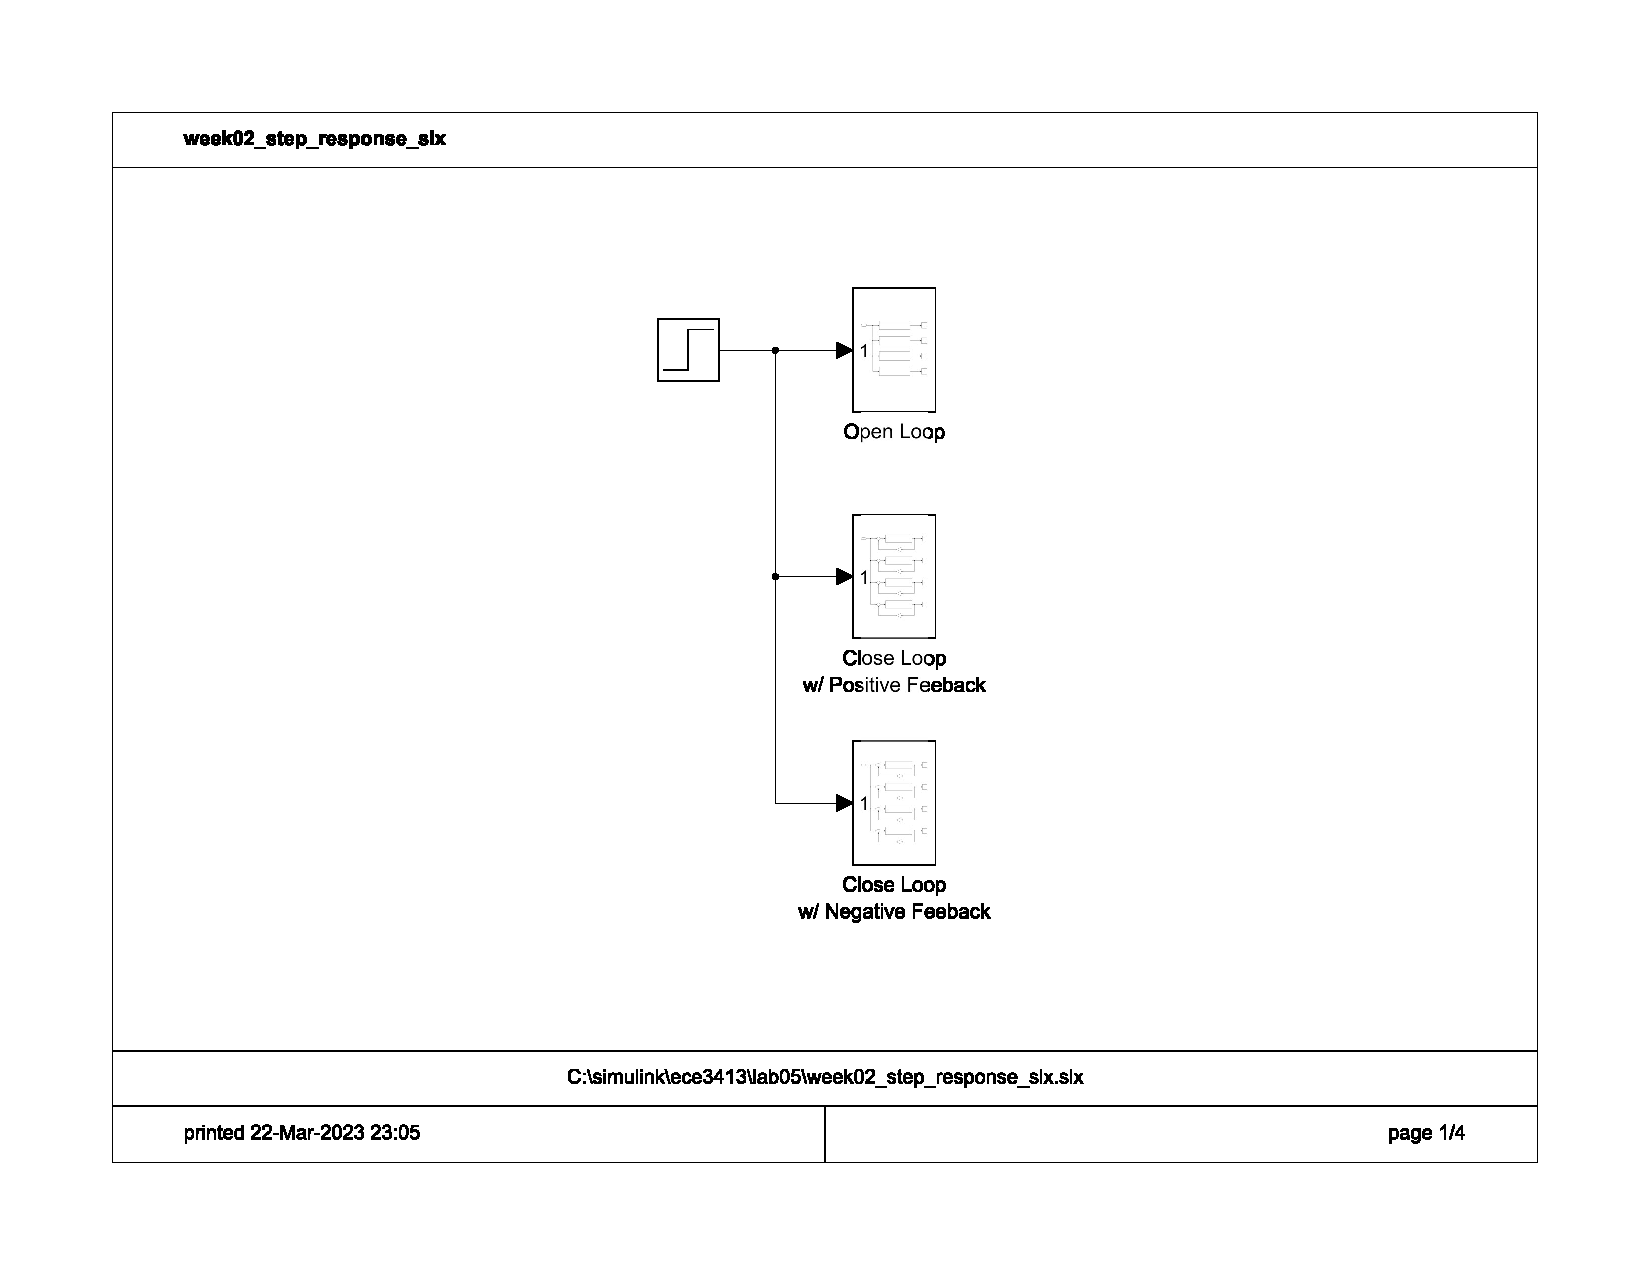
\includepdf[pages=1,landscape=true,pagecommand=\label{pdf:simulink input}]{drawings/week02_step_response_slx.pdf}

\includepdf[pages=4,landscape=true,pagecommand=\label{pdf:open loop}]{drawings/week02_step_response_slx.pdf}

\begin{figure}
    \centering
    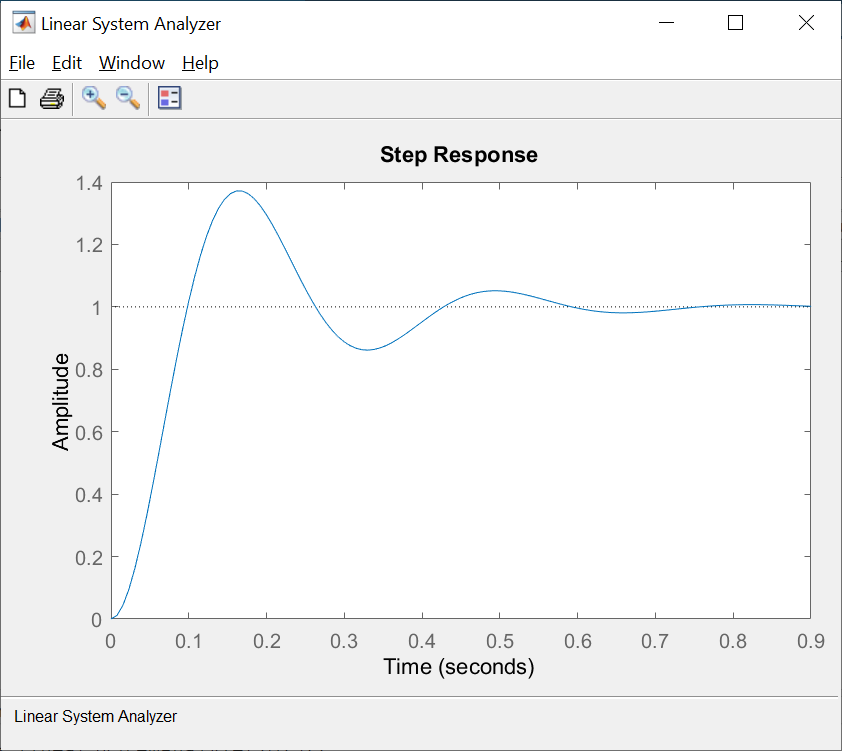
\includegraphics[width=\linewidth]{img/week02-open_loop-g1.png}
    \caption{The step response to the open loop system of transfer function $G_1$.}
    \label{fig:w02 open loop G1}
\end{figure}

To run the Linear System Analyzer on any of these transfer functions, we perform any of the calls
\begin{enumerate}
    \item 
        \mintinline\matlab{linearSystemAnalyzer(G(1))}
    \item 
        \mintinline\matlab{linearSystemAnalyzer(G(2))}
    \item 
        \mintinline\matlab{linearSystemAnalyzer(G(3))}
    \item 
        \mintinline\matlab{linearSystemAnalyzer(G(4))}
\end{enumerate}
respectively in Matlab.

We can see that Fig.~\ref{fig:w02 open loop G1} has an overshoot and oscillates, but eventually settles.
Thus it is underdamped.

\begin{figure}
    \centering
    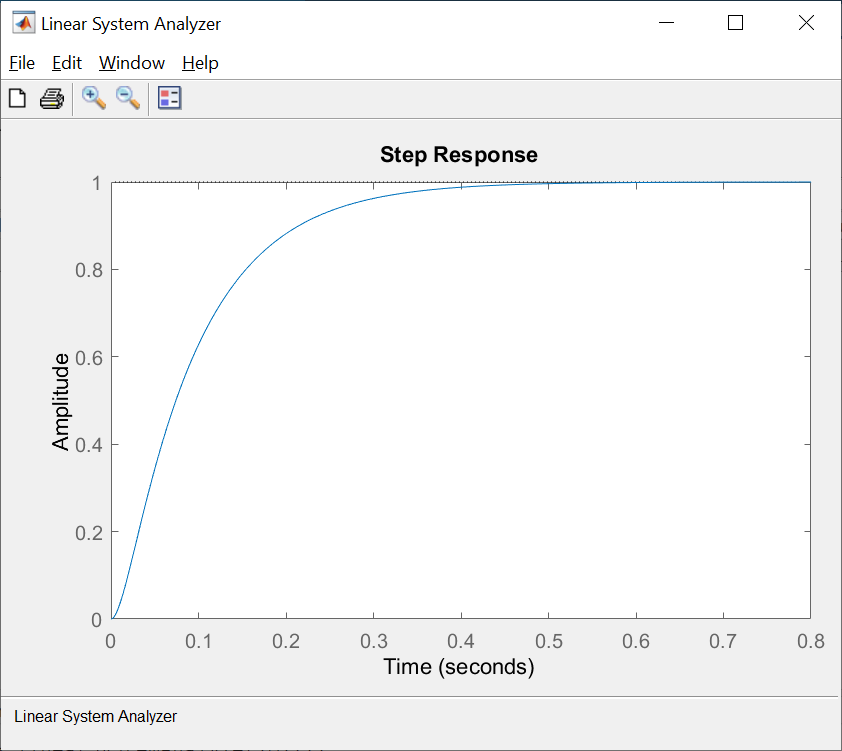
\includegraphics[width=\linewidth]{img/week02-open_loop-g2.png}
    \caption{The step response to the open loop system of transfer function $G_2$.}
    \label{fig:w02 open loop G2}
\end{figure}

We can see that Fig.~\ref{fig:w02 open loop G2} does not overshoot.
It has a fast rise time with a steep slope.
Thus it is critically damped.

\begin{figure}
    \centering
    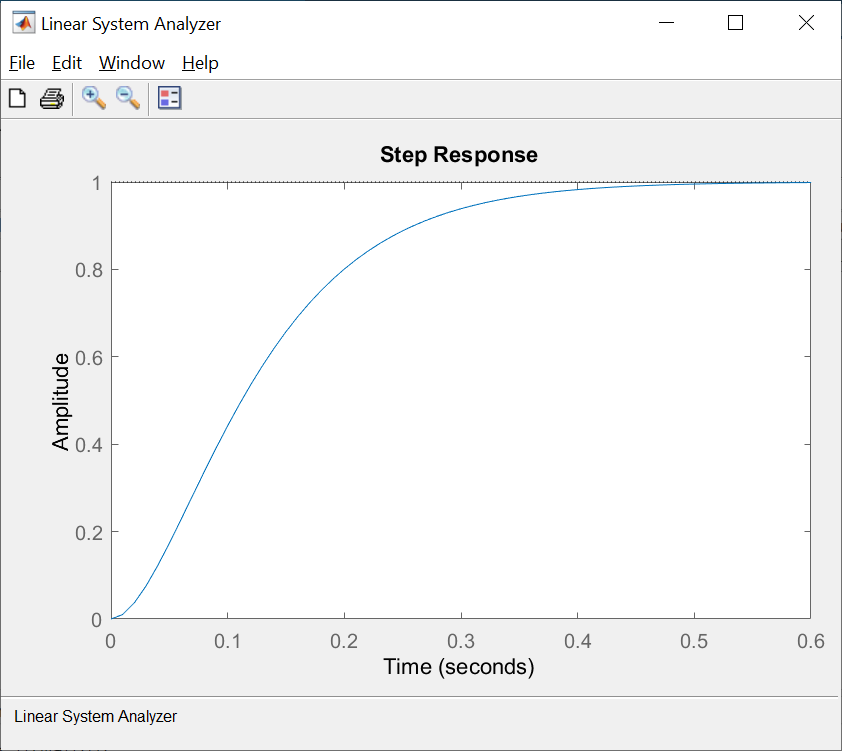
\includegraphics[width=\linewidth]{img/week02-open_loop-g3.png}
    \caption{The step response to the open loop system of transfer function $G_3$.}
    \label{fig:w02 open loop G3}
\end{figure}

We can see that Fig.~\ref{fig:w02 open loop G3} does not overshoot.
It has a slow rise time with a very gradual slope.
Thus it is overdamped.

\begin{figure}
    \centering
    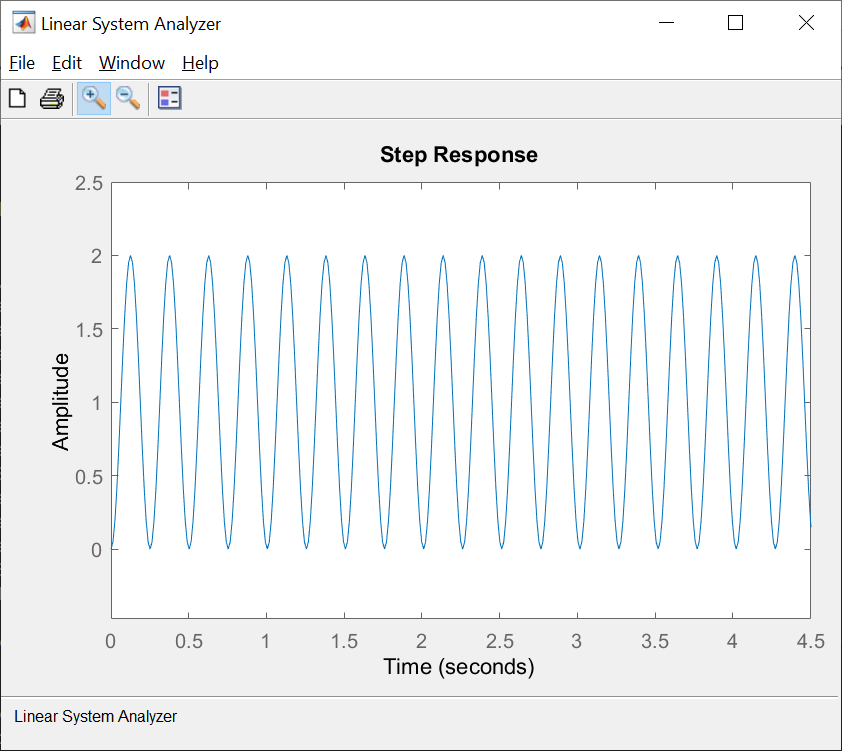
\includegraphics[width=\linewidth]{img/week02-open_loop-g4.png}
    \caption{The step response to the open loop system of transfer function $G_4$.}
    \label{fig:w02 open loop G4}
\end{figure}

We can see that Fig.~\ref{fig:w02 open loop G4} never settles, but rather continues to oscillate forever with no decay.
Thus it is undamped.

\subsection{Week 02, Part 02(a) -- Closed loop with positive feedback}

Next we apply a positive feedback as shown in the model on page~\pageref{pdf:positive feedback}.

To run the Linear System Analyzer on any of these transfer functions, we perform any of the calls

\includepdf[pages=3,landscape=true,pagecommand=\label{pdf:positive feedback}]{drawings/week02_step_response_slx.pdf}

\begin{enumerate}
    \item 
        \mintinline\matlab{k = 1; linearSystemAnalyzer(G(k)/(1 - G(k)*H))}
    \item 
        \mintinline\matlab{k = 2; linearSystemAnalyzer(G(k)/(1 - G(k)*H))}
    \item 
        \mintinline\matlab{k = 3; linearSystemAnalyzer(G(k)/(1 - G(k)*H))}
    \item 
        \mintinline\matlab{k = 4; linearSystemAnalyzer(G(k)/(1 - G(k)*H))}
\end{enumerate}
respectively in Matlab.

\subsection{Week 02, Part 02(b) -- Closed loop with negative feedback}

Finally we change the positive feedback to a positive feedback as shown in the model on page~\pageref{pdf:positive feedback}.

To run the Linear System Analyzer on any of these transfer functions, we perform any of the calls

\begin{enumerate}
    \item 
        \mintinline\matlab{k = 1; linearSystemAnalyzer(G(k)/(1 + G(k)*H))}
    \item 
        \mintinline\matlab{k = 2; linearSystemAnalyzer(G(k)/(1 + G(k)*H))}
    \item 
        \mintinline\matlab{k = 3; linearSystemAnalyzer(G(k)/(1 + G(k)*H))}
    \item 
        \mintinline\matlab{k = 4; linearSystemAnalyzer(G(k)/(1 + G(k)*H))}
\end{enumerate}
respectively in Matlab.

\includepdf[pages=2,landscape=true,pagecommand=\label{pdf:negative feedback}]{drawings/week02_step_response_slx.pdf}

\section{Results}

\subsection{Week 01, Part 01 -- Changing poles}

\begin{figure}
    \centering
    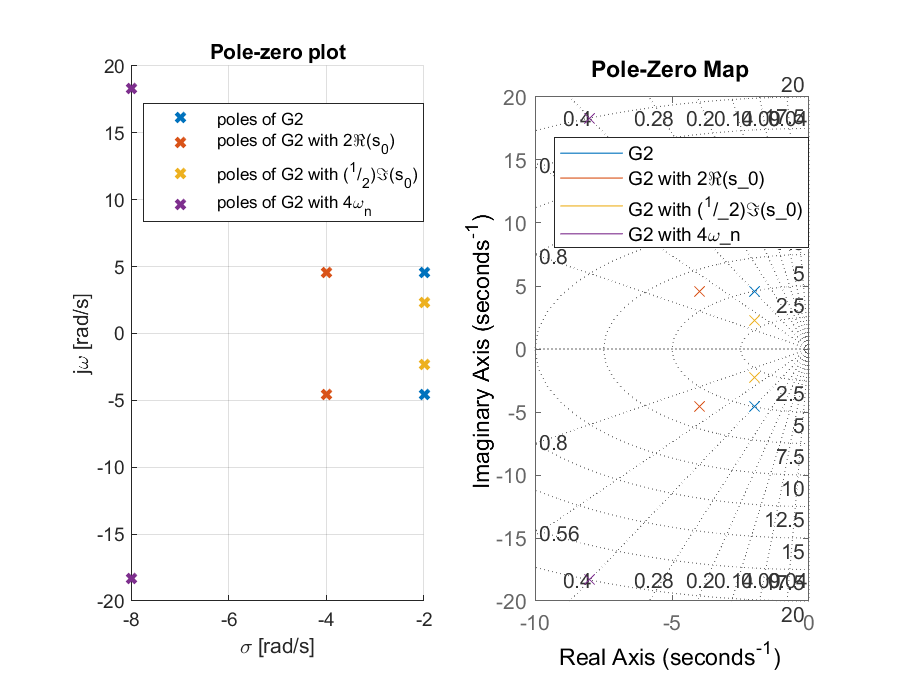
\includegraphics[width=\linewidth]{img/part01_pzplot_pzmap.eps}
    \caption{Comparison pole-zero plot of the transfer functions in Part 01 (subsection~\ref{ssc:part 01}) using a custom plot function that I made on the left available in Appendix subsection~\ref{sap:pzplot}, and using Matlab's built-in \mintinline\matlab{pzmap} on the right.}
    \label{fig:part01_pzplot_pzmap}
\end{figure}

We can see in Fig.~\ref{fig:part01_pzplot_pzmap} that none of the variations of $G_2$ will have zeroes as $G_2$ did not either.

The poles with $\mathfrak{Re}\brao{\setprime{s}_0} = 2\mathfrak{Re}\brao{s_0}$ show that manipulating the real part of the poles scales the $x$-component of the pole.

The poles with $\mathfrak{Im}\brao{\setprime[2]s_0} = \brao*{\sfrac12}\mathfrak{Im}\brao{s_0}$ show that manipulating the imaginary part of the poles scales the $y$-component of the pole.

In the Pole-Zero Map on the right in Fig.~\ref{fig:part01_pzplot_pzmap}, we see that the poles with $\setprime[3]\omega_n = 4\omega_n$ show that manipulating the natural frequency of the transfer function scales the magnitude of the pole.

\begin{table}[]
    \centering
    \caption{Proportional relationships of peak time, overshoot and settling time.}
    \[
        \begin{array}{@{}l*3c@{}}
        \toprule
            \text{parameter}
                & \sfrac{\setprime{T}_p}{T_p}
                & \frac{\log\brao*{\frac{\%\setprime{OS}}{\SI{100}\percent}}}{\log{\brao*{\frac{\%OS^{\vphantom1}}{\SI{100}\percent}}}}
                & \sfrac{\setprime{T}_s}{T_s}
        \\*
        \midrule
            \mathfrak{Re}\brao{\setprime{s}_0} = 2\mathfrak{Re}\brao{s_0}
            & 1
            & 2
            & \sfrac12
        \\*
            \mathfrak{Im}\brao{\setprime{s}_0} = \brao*{\sfrac12}\mathfrak{Im}\brao{s_0}
            & 2
            & 1
            & 1
        \\*
            \setprime\omega_n = 4\omega_n
            & \sfrac14
            & 1
            & \sfrac14
        \\*
        \bottomrule
        \end{array}
    \]
    \label{tab:proportions changing poles}
\end{table}

Table~\ref{tab:proportions changing poles} shows the parameter to modify if we want to change any characteristic of the step response. Particularly, we have shown that
\begin{enumerate}[(a)]
    \addtocounter{enumi}1
    \item
        multiplying the real part exponentiates the overshoot and divides the settling time by the same amount, but does not effect peak time,
    \item
        dividing the imaginary part multiplies the peak time by the same amount, but does not effect overshoot or settling time, and
    \item
        multiplying the natural frequency divides peak time and settling time by the same amount, but does not effect overshoot.
\end{enumerate}

\begin{table}[]
    \centering
    \caption{Numerical comparison of rise times from changing poles.}
    \[
        \begin{array}{@{}>$l<$*3{S@{\,}l}@{}}
        \toprule
            \text{parameter}
                & t_{.9f} & \brac*{\si\second}
                & t_{.1f} & \brac*{\si\second}
                & T_r & \brac*{\si\second}
        \\*
        \midrule
            \text{reference}
            & 0.388761 &
            & 0.096063 &
            & 0.292698
        \\*
        \midrule
            $\mathfrak{Re}\brao{\setprime{s}_0} = 2\mathfrak{Re}\brao{s_0}$
            & 0.411704 &
            & 0.082401 &
            & 0.329303
        \\*
            \%error
            & +5.9016 & \si\percent
            & -14.2219 & \si\percent
            & +12.5061 & \si\percent
        \\*
        \midrule
            $\mathfrak{Im}\brao{\setprime{s}_0} = \brao*{\sfrac12}\mathfrak{Im}\brao{s_0}$
            & 0.823409 &
            & 0.164802 &
            & 0.658607
        \\*
            \%error
            & +111.8034 & \si\percent
            & +71.5562 & \si\percent
            & +125.0125 & \si\percent
        \\*
        \midrule
            $\setprime\omega_n = 4\omega_n$
            & 0.097190 &
            & 0.024016 &
            & 0.073175
        \\*
            \%error
            & -75.0001 & \si\percent
            & -74.9997 & \si\percent
            & -74.9998 & \si\percent
        \\*
        \bottomrule
        \end{array}
    \]
    \label{tab:rise time changing poles}
\end{table}

In Table~\ref{tab:rise time changing poles}, we see that for changing the real part, the upper and lower bounds of the rise time chance in opposite directions (positive and negative respectively). This suggests that manipulating the real part causes a widening of both margins for rise time. For changing the imaginary part, both bounds move up by varying amounts, with the rise time itself growing.

Finally, for the settling frequency, we see both bounds and the rise time itself all move by about the same amount ($\SI{-75.0002}\percent$ by harmonic mean). This seems to be a uniform movement.

\subsection{Week 01, Part 02 -- Adding poles}

\subsubsection{Non-positive real pole with great magnitude}

\begin{figure}
    \centering
    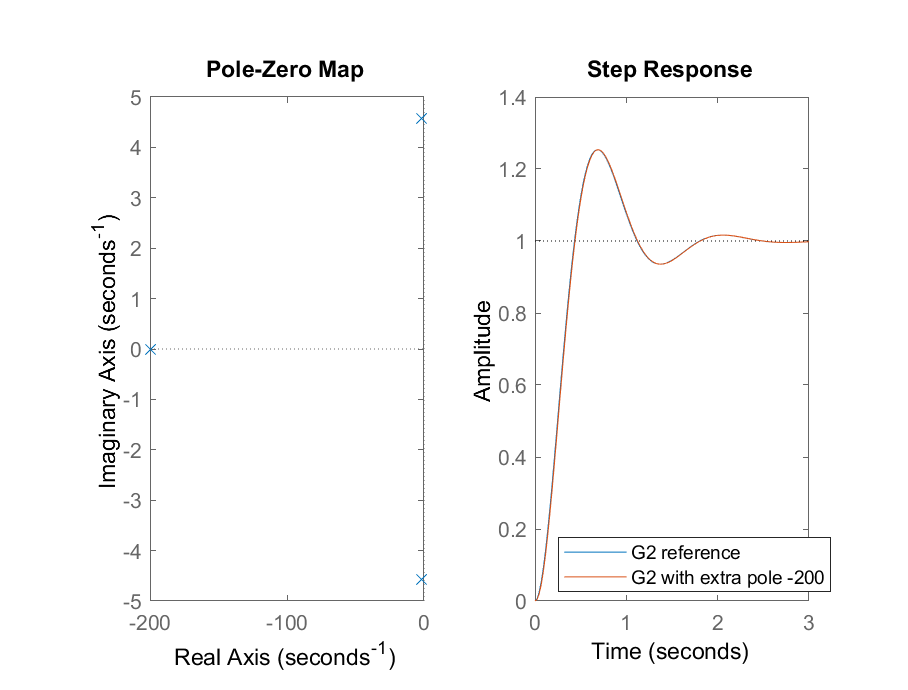
\includegraphics{img/part02_nonpositive_real_pole.eps}
    \caption{The pole-zero map of the new transfer function on the left, and the comparison of the step response of the original reference transfer function $G_2$ and the resulting transfer function of adding non-positive real pole $-\alpha_R = -200$ with great magnitude.}
    \label{fig:non-positive real poles}
\end{figure}

As predicted, we see in Fig.~\ref{fig:non-positive real poles} that the resulting transfer function is very close to the original reference transfer function.

\begin{table}[]
    \centering
    \caption{Numerical comparison of reference function and the result of adding the pole $-\alpha_R$.}
    \[
        \begin{array}{@{}>$l<$*4{S@{\,}l}@{}}
        \toprule
            name &
            T_p\ & \brac*{\si\second}
                & \%OS &
                & T_s & \brac*{\si\second}
                & T_r & \brac*{\si\second}
        \\*
        \midrule
            reference &
            0.6856 && 25.3802 & \si\percent & 2 && 0.292698
        \\*
            $-\alpha_R$ &
            0.6908 && 25.3746 & \si\percent & 1.6870 && 0.2934
        \\*
        \midrule
            \%error &
            -0.7528 & \si\percent
                & +0.0221 & \si\percent
                & +18.5536 & \si\percent
                & -0.2393 & \si\percent
        \\*
        \bottomrule
        \end{array}
    \]
    \label{tab:non-positive real poles}
\end{table}

To find the transient response of the $3^{\text{{o}}}$ transfer function,
we will use the Matlab function \mintinline\matlab{stepinfo} because we do not have formulas to find the exact values as we did for $2^{\text{{o}}}$ underdamped systems.

Furthermore, Table~\ref{tab:non-positive real poles} shows satisfactory errors for peak time, rate of overshoot and rise time.
However, the difference for the settling time is quite high at $\SI{18.5}\percent$. Since Fig.~\ref{fig:non-positive real poles} is such a close fit, I believe that this may be due to differing definitions of the settling time. Both \citet{nise2015a} and \citet{matlab2022a} use a $\SI2\percent$ settling time. However, the difference may come down to the formula from \citet{nise2015a} assuming a settling time from above and \citet{matlab2022a} assuming a settling time from below.

\subsubsection{Positive real pole}

\begin{figure}
    \centering
    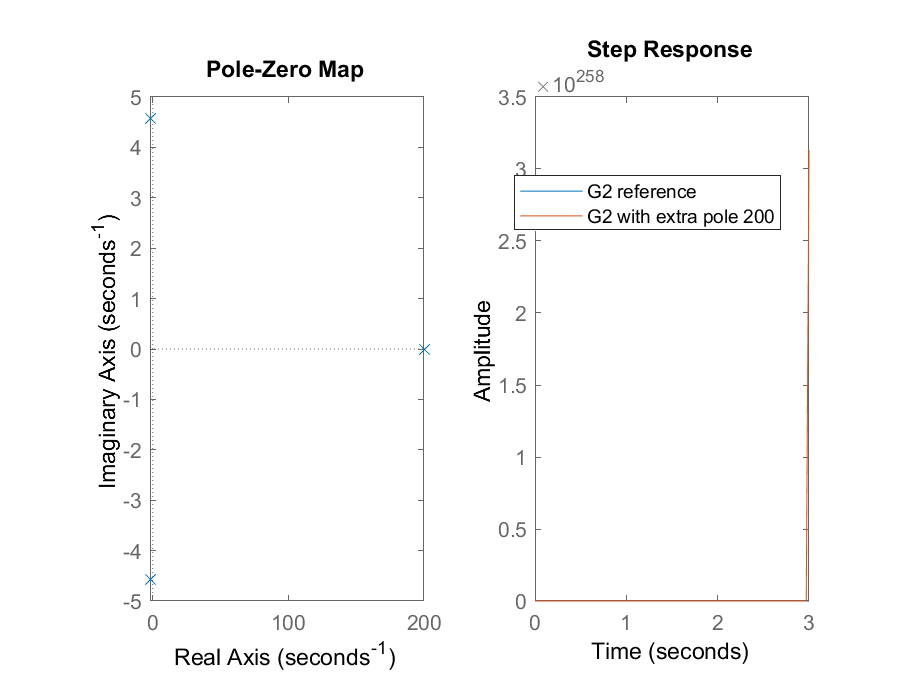
\includegraphics{img/part02_positive_real_pole.eps}
    \caption{The pole-zero map of the new transfer function on the left, and the comparison of the step response of the original reference transfer function $G_2$ and the resulting transfer function of adding positive real pole $\alpha_R = 200$.}
    \label{fig:positive real poles}
\end{figure}

In this case, we saw the transfer function grow to \num{3.5e+258}, which would trend to positive infinity. Just as predicted, this shows that the new transfer function is unstable.

Further inspection of Table~\ref{tab:positive real poles} shows that the step response has infinite peak time, indeterminate rate of overshoot, settling time and rise time. This is expected because the peak is never reached. As such the peak time would be infinite. The overshoot, settling time and rise time are questions that do not make sense without a possible final value.

\begin{table}[]
    \centering
    \caption{Numerical comparison of reference function and the result of adding the pole $+\alpha_R$.}
    \[
        \begin{array}{@{}>$l<$*4S@{}}
        \toprule
            name &
            T_p\ \brac*{\si\second}
                & \%OS
                & T_s\ \brac*{\si\second}
                & T_r\ \brac*{\si\second}
        \\*
        \midrule
            reference &
            0.6856 & \SI{25.3802}\percent & 2 & 0.292698
        \\*
            $+\alpha_R$ &
            \text{$+\infty$} & \text{---} & \text{---} & \text{---}
        \\*
        \midrule
            \%error &
            \frac\infty\infty
                & \text{---}
                & \text{---}
                & \text{---}
        \\*
        \bottomrule
        \end{array}
    \]
    \label{tab:positive real poles}
\end{table}

\subsection{Week 02, Part 01}

\subsection{Week 02, Part 02(a) -- Closed loop with positive feedback}

From the Simulink Model on page~\pageref{pdf:positive feedback}
we build the Fig.~\ref{fig:w02 positive feedback G1}, Fig.~\ref{fig:w02 positive feedback G2}, Fig.~\ref{fig:w02 positive feedback G3} and Fig.~\ref{fig:w02 positive feedback G4}.

\begin{figure}
    \centering
    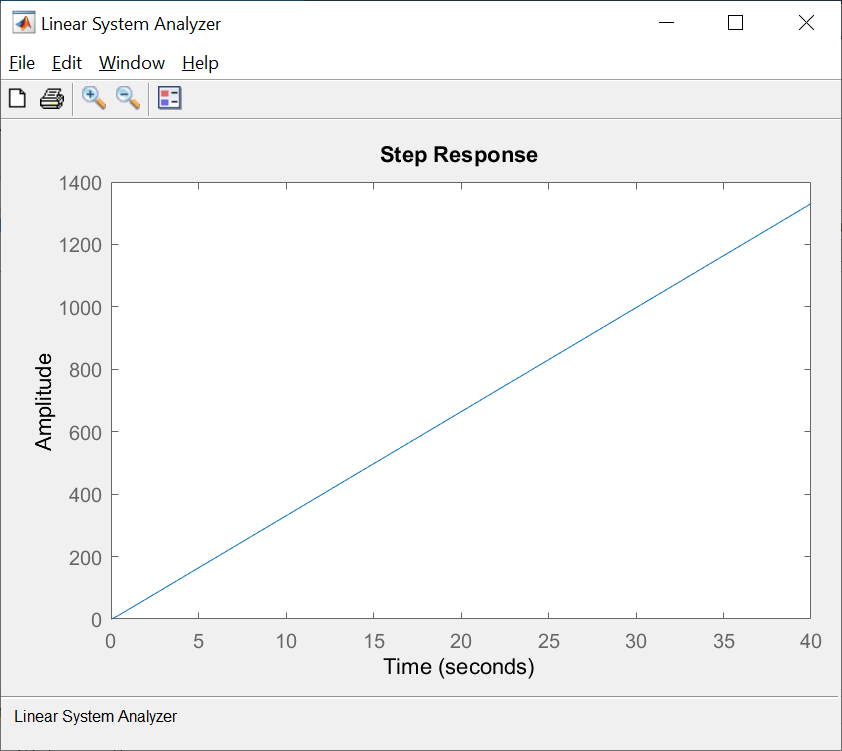
\includegraphics[width=\linewidth]{img/week02-positive_feedback-g1.png}
    \caption{The step response to the positive feedback, close loop system of transfer function $G_1$.}
    \label{fig:w02 positive feedback G1}
\end{figure}

The step response of the positive feedback of underdamped system with transfer function $G_1$ appears to be a ramp function.

\begin{figure}
    \centering
    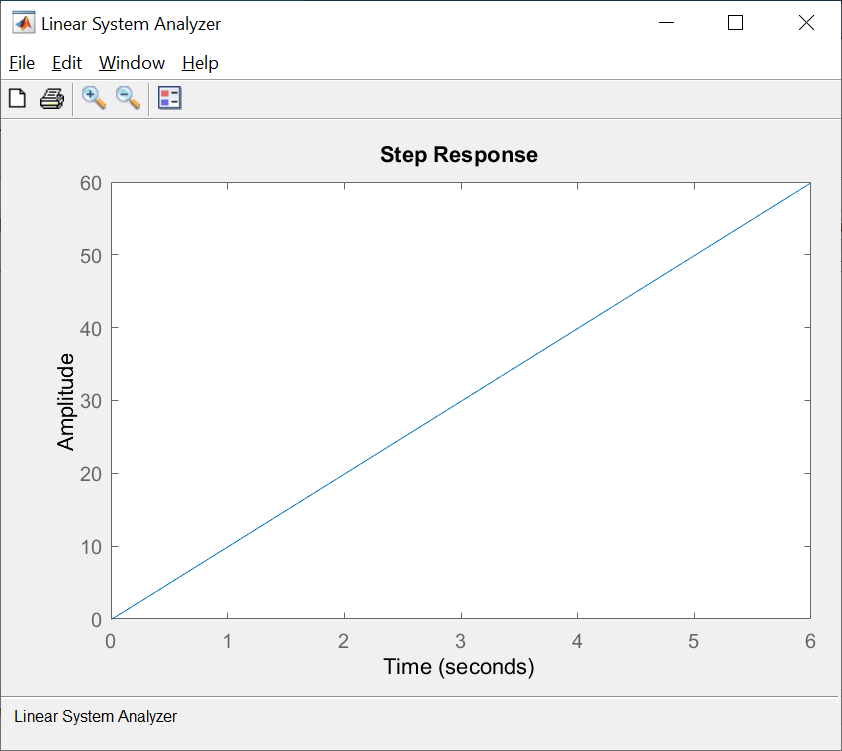
\includegraphics[width=\linewidth]{img/week02-positive_feedback-g2.png}
    \caption{The step response to the positive feedback, close loop system of transfer function $G_2$.}
    \label{fig:w02 positive feedback G2}
\end{figure}

The step response of the positive feedback of critically damped system with transfer function $G_2$ appears to be a ramp function.

\begin{figure}
    \centering
    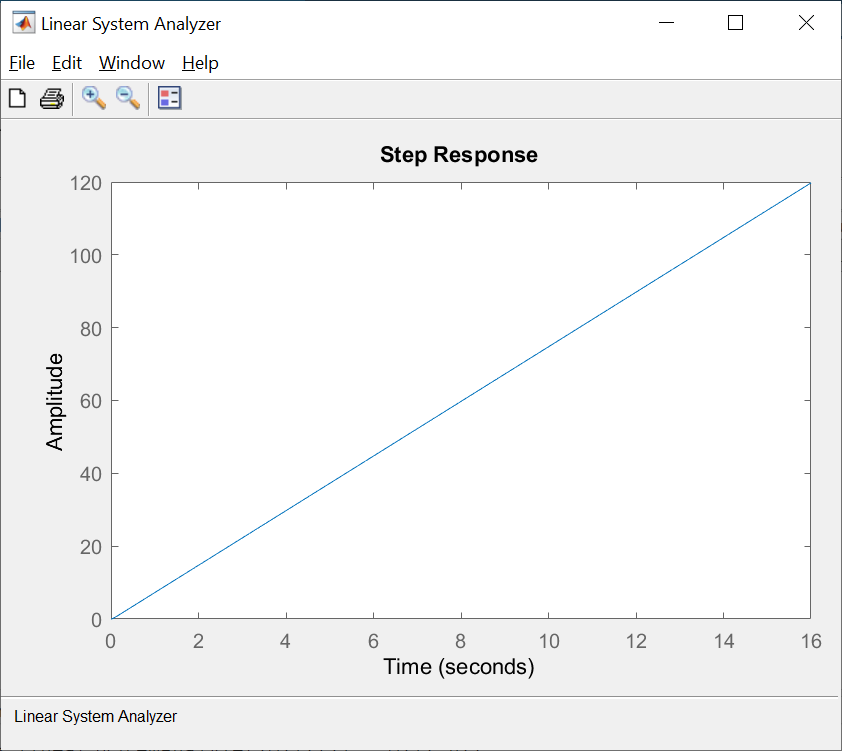
\includegraphics[width=\linewidth]{img/week02-positive_feedback-g3.png}
    \caption{The step response to the positive feedback, close loop system of transfer function $G_3$.}
    \label{fig:w02 positive feedback G3}
\end{figure}

The step response of the positive feedback of overdamped system with transfer function $G_3$ appears to be a ramp function.

\begin{figure}
    \centering
    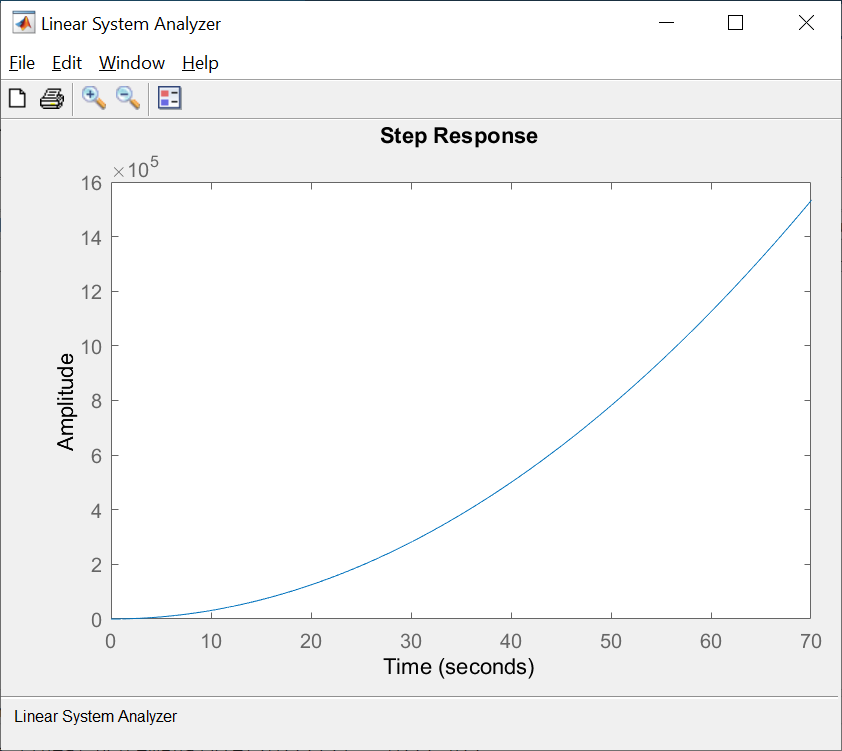
\includegraphics[width=\linewidth]{img/week02-positive_feedback-g4.png}
    \caption{The step response to the positive feedback, close loop system of transfer function $G_4$.}
    \label{fig:w02 positive feedback G4}
\end{figure}

The step response of the positive feedback of undamped system with transfer function $G_4$ is a concave up function that appears to be a geometric growth function.

\subsection{Week 02, Part 02(a) -- Closed loop with negative feedback}

From the Simulink Model on page~\pageref{pdf:negative feedback}
we build the Fig.~\ref{fig:w02 negative feedback G1}, Fig.~\ref{fig:w02 negative feedback G2}, Fig.~\ref{fig:w02 negative feedback G3} and Fig.~\ref{fig:w02 negative feedback G4}.

\begin{figure}
    \centering
    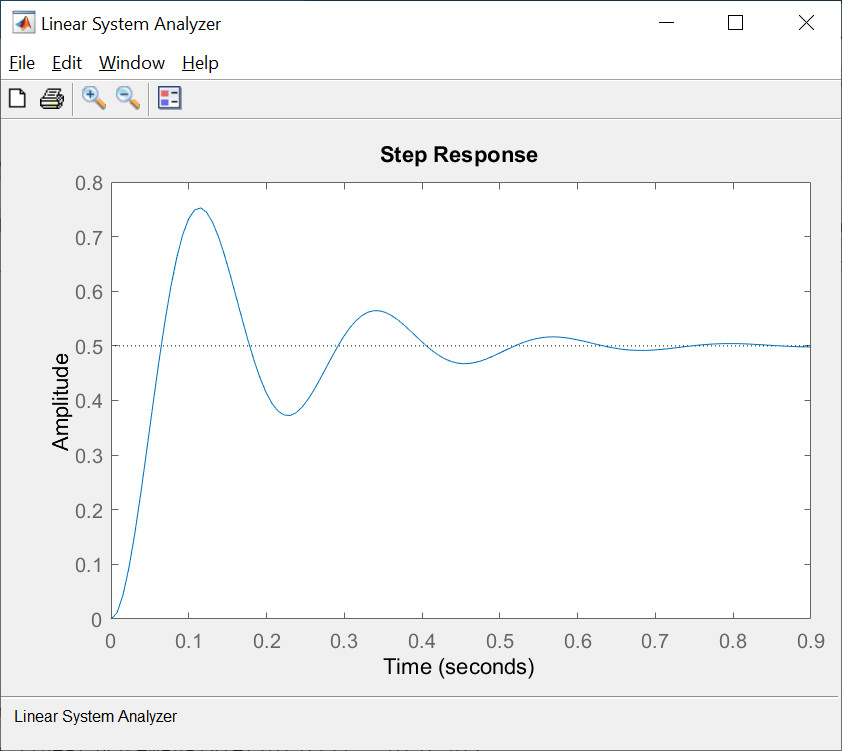
\includegraphics[width=\linewidth]{img/week02-negative_feedback-g1.png}
    \caption{The step response to the negative feedback, close loop system of transfer function $G_1$.}
    \label{fig:w02 negative feedback G1}
\end{figure}

The step response of the negative feedback of underdamped system with transfer function $G_1$ is also an underdamped system.

\begin{figure}
    \centering
    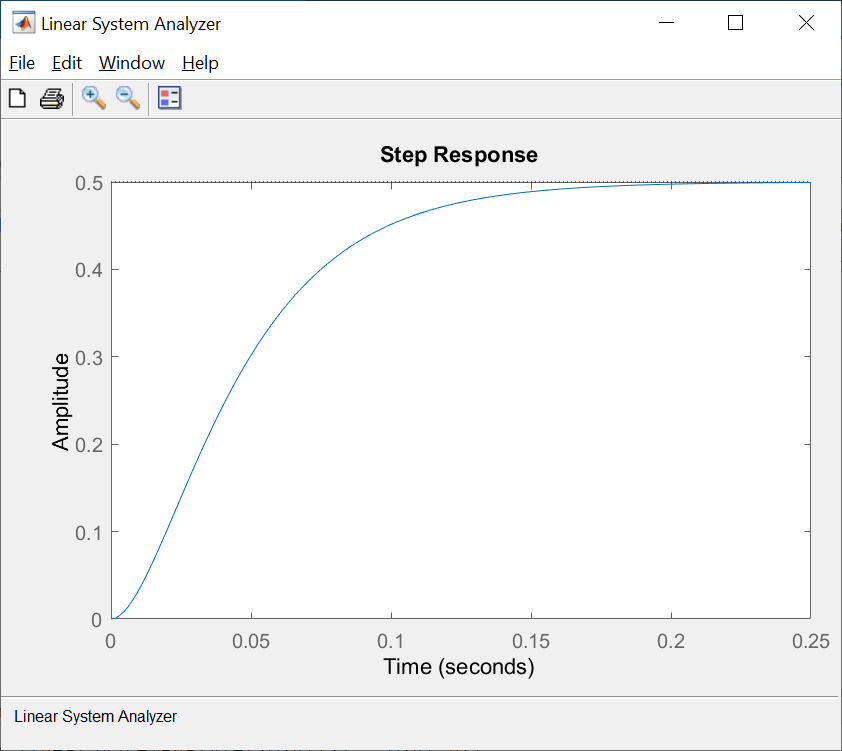
\includegraphics[width=\linewidth]{img/week02-negative_feedback-g2.png}
    \caption{The step response to the negative feedback, close loop system of transfer function $G_2$.}
    \label{fig:w02 negative feedback G2}
\end{figure}

The step response of the negative feedback of critically damped system with transfer function $G_2$ is an overdamped system as can be seen by its more graduate rise time slope.

\begin{figure}
    \centering
    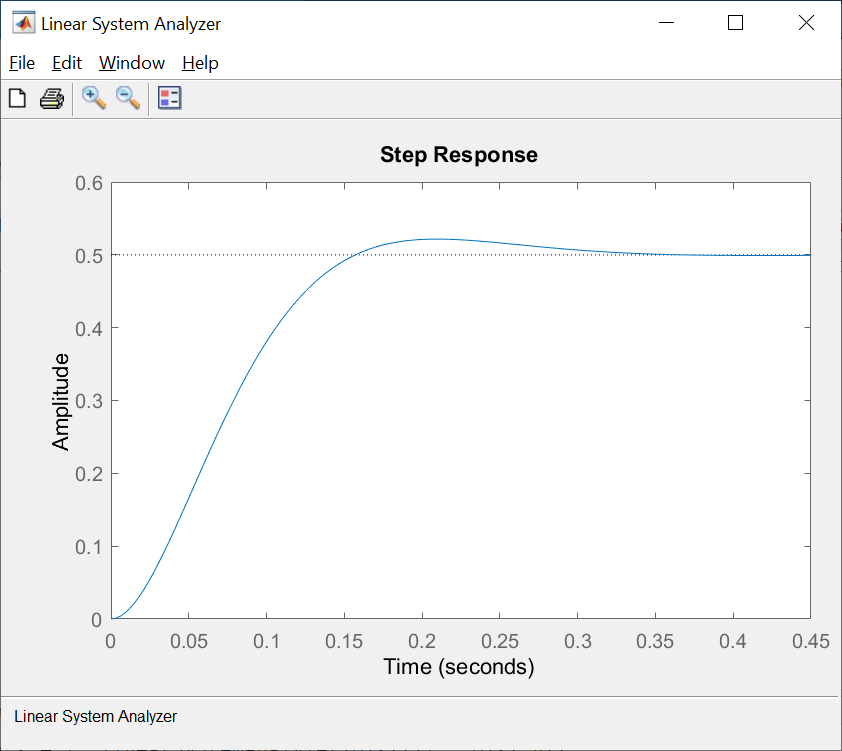
\includegraphics[width=\linewidth]{img/week02-negative_feedback-g3.png}
    \caption{The step response to the negative feedback, close loop system of transfer function $G_3$.}
    \label{fig:w02 negative feedback G3}
\end{figure}

The step response of the negative feedback of overdamped system with transfer function $G_3$ is an underdamped system as can be seen by its slight overshoot.

\begin{figure}
    \centering
    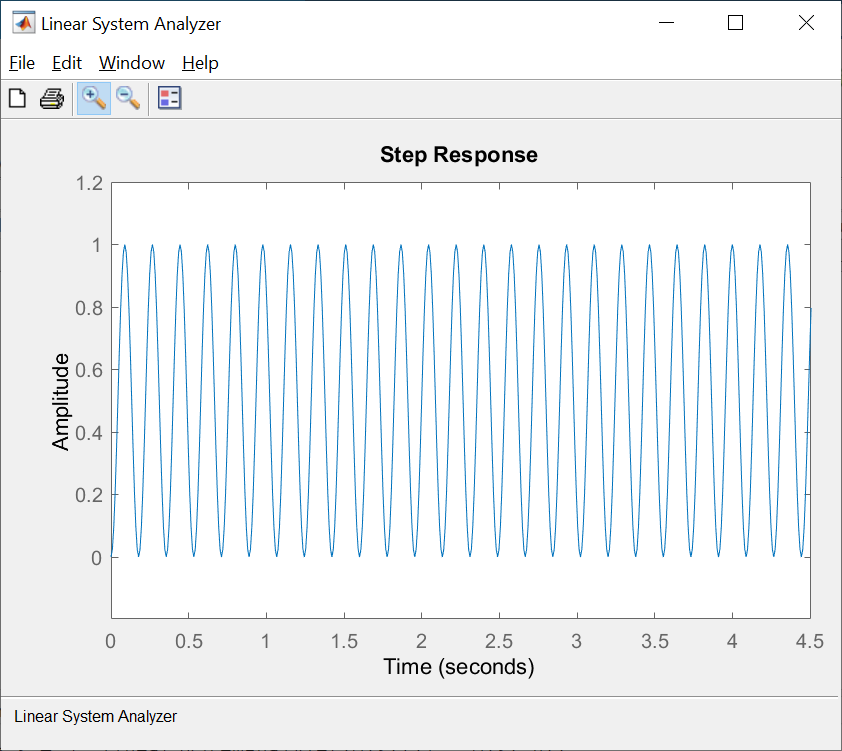
\includegraphics[width=\linewidth]{img/week02-negative_feedback-g4.png}
    \caption{The step response to the negative feedback, close loop system of transfer function $G_4$.}
    \label{fig:w02 negative feedback G4}
\end{figure}

The step response of the negative feedback of undamped system with transfer function $G_3$ is still undamped.

\section{Discussion}

\paragraph{For week 01}

In this lab, we learned that manipulating the real and imaginary parts of the poles will effect their $x$- and $y$-components respectively, and that manipulating the natural frequency will effect the poles' magnitudes.

Regarding this, I learned that graphing in the polar co\"ordinate system is not as well supported by Matlab as the Cartesian co\"ordinate system.
There is a \mintinline\matlab{polarplot} function.
However it does not support multiple plots and cannot be combined with a plot in Cartesian.
Because of this, going forward, I will use \mintinline\matlab{pzmap} instead;
and if I need to use the more primitive facilities of polar co\"ordinate system,
then I will have to prefer to find an alternative system such as Python.


This lab also gave us the opportunity to test the hypothesis that a positive real pole will always be result in an unstable transfer function, whereas a transfer function where all poles only have non-positive real part will be stable.
Additionally, we have learned that the poles with real part closest to $0$ dominate.
It is also a good time to remember that a pole that has $5\times$ the real part $-\zeta\omega_n$ of another pole
will have very little significant effect in comparison.
This former pole is $5\tau$ away from the latter pole.

Now we can see that the rise time has no direct relationship with the roots or the natural frequency.
Because of this, we had to use the Matlab equation solver to find the appropriate times at $\SI{10}\percent$ and $\SI{90}\percent$ final output,
and from this calculate the rise times.

From Table~\ref{tab:rise time changing poles}, we can confirm no obvious relation for the components of the pole. However, there seems to be a scaling effect to the natural frequency. Let's investigate further.

\begin{figure}
    \centering
    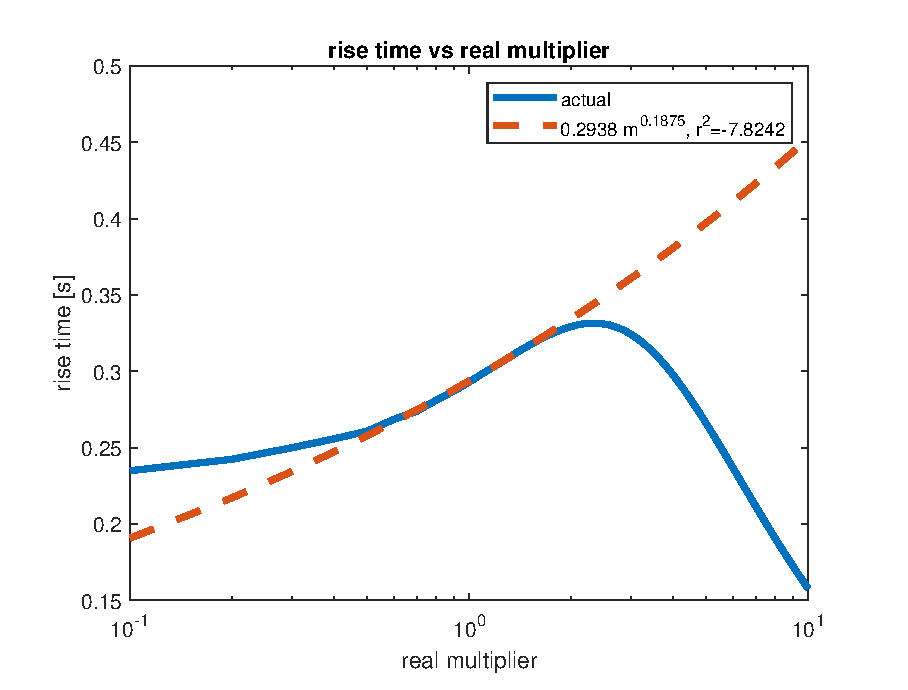
\includegraphics[width=\linewidth]{img/part01_rise_time_vs_real.eps}
    \caption{Plot in a semi-log scale on the $x$-axis
    showing the effect of multiplying the real component of the poles on the rise time and log-log linear regression.}
    \label{fig:rise time vs real}
\end{figure}

The script in Appendix subsection~\ref{sap:rise time vs parameters}
plots the rise time vs the parameters that we have investigated
in a semi-log scale on the $x$-axis
from the reciprocal of the modification to the modification.
(For the imaginary part, this is the reverse because the modification was scaling by $\sfrac12$.)
A log-log linear regression is taken from these, and then the entire plot is scaled by $5$ on each side
to allow for scaling.

This produces Fig.~\ref{fig:rise time vs real}, \ref{fig:rise time vs imag} and \ref{fig:rise time vs wn}.

\paragraph{Note that} since the Matlab equation solver is time expensive and each plot will use $100$ samples, we use the Matlab \mintinline\matlab{stepinfo} function to find the rise time, albeit it does not the bounds of the rise time.

\begin{figure}
    \centering
    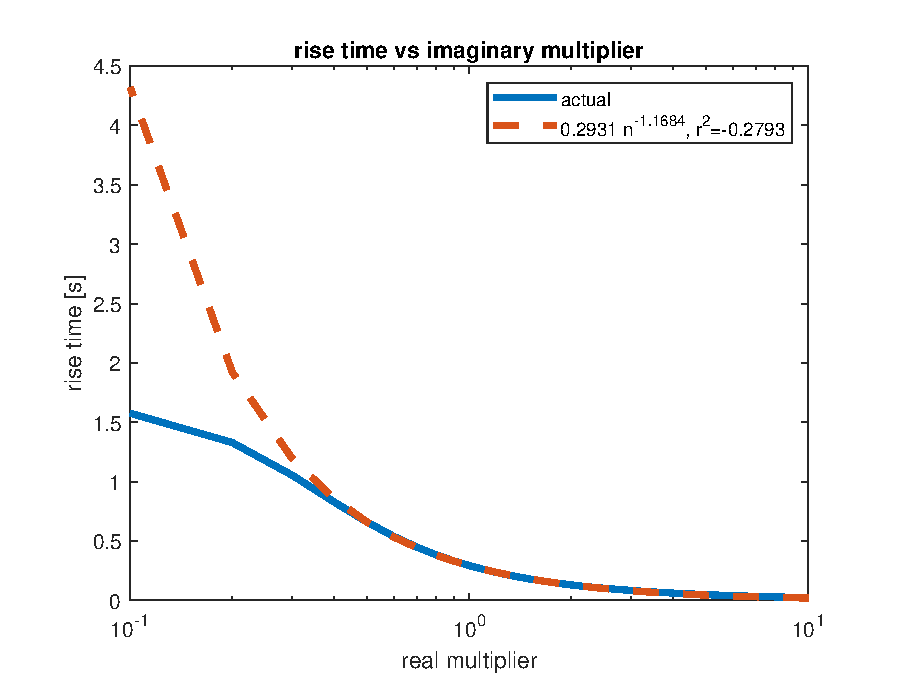
\includegraphics[width=\linewidth]{img/part01_rise_time_vs_imag.eps}
    \caption{Plot in a semi-log scale on the $x$-axis
    showing the effect of multiplying the imaginary component of the poles on the rise time and log-log linear regression.}
    \label{fig:rise time vs imag}
\end{figure}

Now, the coefficients in $\brac{\begin{matrix}0.2938 & 0.2931 & 0.2930\end{matrix}}$ represent the rise time of the original transfer function,
which we found to be \SI{0.292698}\second in sub-subsection~\ref{sss:evaluations}.
These values represent that rise time with deviation $\num{0.00085651}$.

For modifying the real component, the linear regression
(in Fig.~\ref{fig:rise time vs real})
was only successful locally at $\brac{0.3, 2.3}$ with $r^2 = \num{0.956348}$.
Thus, there does not seem to be a relation between the real component and rise time.

\begin{figure}
    \centering
    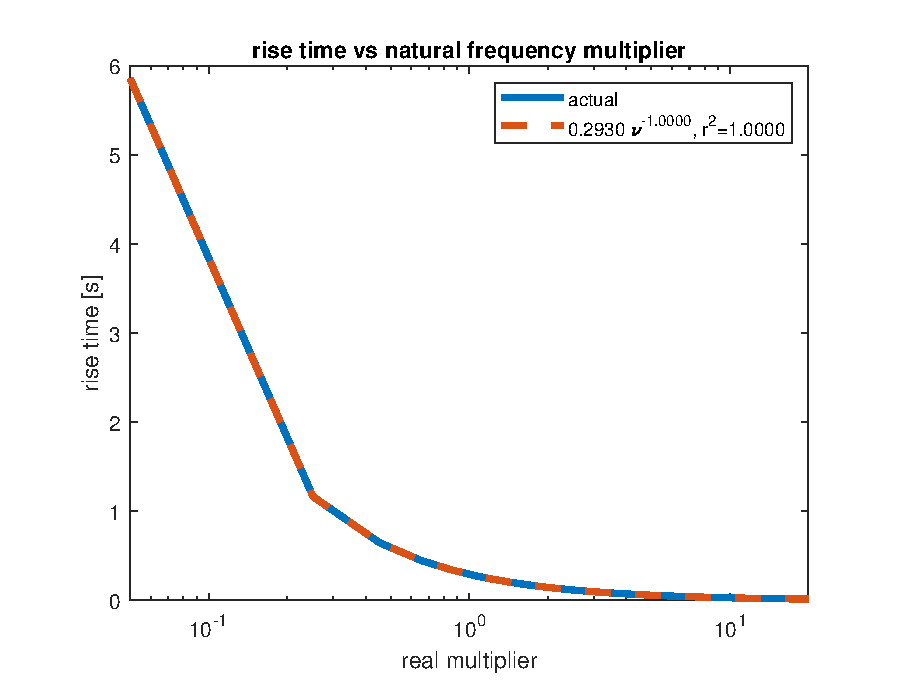
\includegraphics[width=\linewidth]{img/part01_rise_time_vs_wn.eps}
    \caption{Plot in a semi-log scale on the $x$-axis
    showing the effect of multiplying the natural frequency on the rise time and log-log linear regression.}
    \label{fig:rise time vs wn}
\end{figure}

For modifying the imaginary component, the linear regression
(in Fig.~\ref{fig:rise time vs imag})
is much better, having $r^2 = 0.991558$ in $\brac{0.3, 9.8}$.
I predict that after $n = 0.3$, the effect of multiplying the imaginary part by imaginary part of the pole by $n$ will result in a division of the rise time by $n^{1.1684}$.
In fact, taking the original rise time \SI{0.292698}\second and dividing by $\brao*{\sfrac12}^1.1684$ gives $\SI{0.657874}\second$.
The calculated value for the rise time halving the imaginary part of the pole was $\SI{0.658607}\second$.
That's a rate of error of $\SI{-0.111295}\percent$.
Interestingly since the modification was to half the imaginary part, this prediction may not be so useful.

Earlier, we speculated that modifying the natural frequency uniformly moves the range of the rise time.
In Fig.~\ref{fig:rise time vs wn}, we find an $r^2 = 1.0000$ from $\brao{0.05, 19.3955}$.
This appears to be an exact match!
We can predict that multiplying the natural frequency by $\nu$ will result in dividing the rise time by $\nu$.
Now
\begin{equation}
    \frac{T_r}\nu = \frac{\SI{0.292698}\second}4 = \SI{0.0731745}\second \approx \SI{0.073175}\second = \setprime[3]{T}_r
\end{equation}
with a negligible $\SI{-6.83293e-6}{\second^0}$ rate of error.

Moreover, it the natural frequency
scales the time domain
of a transfer function.
Earlier we saw that changing the natural frequency $\setprime\omega_n = \nu\omega_n$ results in
new peak time $\setprime{T}_p = \sfrac{T_p}\nu$ and
new settling time $\setprime{T}_s = \sfrac{T_s}\nu$,
and now we have the relation $\setprime{T}_r = \sfrac{T_r}\nu$
as well as the bounds $\setprime{t}_{.9f} = \sfrac{t_{.9f}}\nu,\ \setprime{t}_{.1f} = \sfrac{t_{.1f}}\nu$
from Table~\ref{tab:rise time changing poles}.
In the case of overshoot, it makes sense that this would not be affected
as overshoot is a characteristic of the range of step response, not the domain.

Thus, we see that generally it is the case that if $c$ is a transfer function with natural frequency $\omega_n$
and $\setprime{c}$ is a transfer function that is almost equivalent, but with natural frequency $\nu\omega_n$,
then
\begin{equation}
    \setprime{c}\brao*{\frac{t}\nu} = c\brao*t.
\end{equation}

\paragraph{For week 02}

We see the effect of the poles on the dampening of the system.

We see that stable systems always have poles in the left half plane, overdamped systems are produced by two complex poles, overdamped systems are produced by two unique real roots, critically damped systems are produced by a double real root and undamped systems are produced by imaginary roots.

The positive feedback always seems to create unstable systems, whereas negative feedback produced similar stable systems that may differ in damping.

\newpage
\printbibliography

\newpage
\appendix
\section{Appendix}

\subsection{Week 01, Part 01 -- Rise time, Matlab script}\label{sap:solving for .9cf and .1cf}
\inputminted{matlab}{src/part01a_rise_time.m}

\subsection{Week 01, Part 01 -- Pole-zero plot, Matlab Live Script}\label{sap:pzplot}
\inputminted{matlab}{src/part01a_pzplot_mlx.m}

\subsection{Week 01, Part 02 -- Comparing results of adding poles, Matlab Script}\label{sap:adding poles}
\inputminted{matlab}{src/part02_adding_poles.m}

\subsection{Week 01, Part 01 Discussion -- Plotting rise time vs parameters, Matlab Script}\label{sap:rise time vs parameters}
\inputminted{matlab}{src/part01_rise_time_vs_parameters_plot.m}

\subsection{Week 02, Part 01 -- Simulation parameters, Matlab script}\label{sap:params}
\inputminted{matlab}{src/week02_simulation_params.m}

\subsection{Week 02, Part 01 -- Pole-zero plot, Matlab script}\label{sap:pzplot 2}
\inputminted{matlab}{src/week02_part01_pzplot.m}

\subsection{Multiset constructor, Matlab function}\label{sap:multiset}
\inputminted{matlab}{src/multiset.m}

\end{document}
